\PassOptionsToPackage{unicode=true}{hyperref} % options for packages loaded elsewhere
\PassOptionsToPackage{hyphens}{url}
%
\documentclass[]{book}
\usepackage{lmodern}
\usepackage{amssymb,amsmath}
\usepackage{ifxetex,ifluatex}
\usepackage{fixltx2e} % provides \textsubscript
\ifnum 0\ifxetex 1\fi\ifluatex 1\fi=0 % if pdftex
  \usepackage[T1]{fontenc}
  \usepackage[utf8]{inputenc}
  \usepackage{textcomp} % provides euro and other symbols
\else % if luatex or xelatex
  \usepackage{unicode-math}
  \defaultfontfeatures{Ligatures=TeX,Scale=MatchLowercase}
\fi
% use upquote if available, for straight quotes in verbatim environments
\IfFileExists{upquote.sty}{\usepackage{upquote}}{}
% use microtype if available
\IfFileExists{microtype.sty}{%
\usepackage[]{microtype}
\UseMicrotypeSet[protrusion]{basicmath} % disable protrusion for tt fonts
}{}
\IfFileExists{parskip.sty}{%
\usepackage{parskip}
}{% else
\setlength{\parindent}{0pt}
\setlength{\parskip}{6pt plus 2pt minus 1pt}
}
\usepackage{hyperref}
\hypersetup{
            pdftitle={BASS4 - ADMINISTRATOR'S MANUAL},
            pdfauthor={Louise Serenhov, Erik Sjöstrand, Jenny-Li Örsell \& Brjánn Ljótsson},
            pdfborder={0 0 0},
            breaklinks=true}
\urlstyle{same}  % don't use monospace font for urls
\usepackage{color}
\usepackage{fancyvrb}
\newcommand{\VerbBar}{|}
\newcommand{\VERB}{\Verb[commandchars=\\\{\}]}
\DefineVerbatimEnvironment{Highlighting}{Verbatim}{commandchars=\\\{\}}
% Add ',fontsize=\small' for more characters per line
\usepackage{framed}
\definecolor{shadecolor}{RGB}{248,248,248}
\newenvironment{Shaded}{\begin{snugshade}}{\end{snugshade}}
\newcommand{\AlertTok}[1]{\textcolor[rgb]{0.94,0.16,0.16}{#1}}
\newcommand{\AnnotationTok}[1]{\textcolor[rgb]{0.56,0.35,0.01}{\textbf{\textit{#1}}}}
\newcommand{\AttributeTok}[1]{\textcolor[rgb]{0.77,0.63,0.00}{#1}}
\newcommand{\BaseNTok}[1]{\textcolor[rgb]{0.00,0.00,0.81}{#1}}
\newcommand{\BuiltInTok}[1]{#1}
\newcommand{\CharTok}[1]{\textcolor[rgb]{0.31,0.60,0.02}{#1}}
\newcommand{\CommentTok}[1]{\textcolor[rgb]{0.56,0.35,0.01}{\textit{#1}}}
\newcommand{\CommentVarTok}[1]{\textcolor[rgb]{0.56,0.35,0.01}{\textbf{\textit{#1}}}}
\newcommand{\ConstantTok}[1]{\textcolor[rgb]{0.00,0.00,0.00}{#1}}
\newcommand{\ControlFlowTok}[1]{\textcolor[rgb]{0.13,0.29,0.53}{\textbf{#1}}}
\newcommand{\DataTypeTok}[1]{\textcolor[rgb]{0.13,0.29,0.53}{#1}}
\newcommand{\DecValTok}[1]{\textcolor[rgb]{0.00,0.00,0.81}{#1}}
\newcommand{\DocumentationTok}[1]{\textcolor[rgb]{0.56,0.35,0.01}{\textbf{\textit{#1}}}}
\newcommand{\ErrorTok}[1]{\textcolor[rgb]{0.64,0.00,0.00}{\textbf{#1}}}
\newcommand{\ExtensionTok}[1]{#1}
\newcommand{\FloatTok}[1]{\textcolor[rgb]{0.00,0.00,0.81}{#1}}
\newcommand{\FunctionTok}[1]{\textcolor[rgb]{0.00,0.00,0.00}{#1}}
\newcommand{\ImportTok}[1]{#1}
\newcommand{\InformationTok}[1]{\textcolor[rgb]{0.56,0.35,0.01}{\textbf{\textit{#1}}}}
\newcommand{\KeywordTok}[1]{\textcolor[rgb]{0.13,0.29,0.53}{\textbf{#1}}}
\newcommand{\NormalTok}[1]{#1}
\newcommand{\OperatorTok}[1]{\textcolor[rgb]{0.81,0.36,0.00}{\textbf{#1}}}
\newcommand{\OtherTok}[1]{\textcolor[rgb]{0.56,0.35,0.01}{#1}}
\newcommand{\PreprocessorTok}[1]{\textcolor[rgb]{0.56,0.35,0.01}{\textit{#1}}}
\newcommand{\RegionMarkerTok}[1]{#1}
\newcommand{\SpecialCharTok}[1]{\textcolor[rgb]{0.00,0.00,0.00}{#1}}
\newcommand{\SpecialStringTok}[1]{\textcolor[rgb]{0.31,0.60,0.02}{#1}}
\newcommand{\StringTok}[1]{\textcolor[rgb]{0.31,0.60,0.02}{#1}}
\newcommand{\VariableTok}[1]{\textcolor[rgb]{0.00,0.00,0.00}{#1}}
\newcommand{\VerbatimStringTok}[1]{\textcolor[rgb]{0.31,0.60,0.02}{#1}}
\newcommand{\WarningTok}[1]{\textcolor[rgb]{0.56,0.35,0.01}{\textbf{\textit{#1}}}}
\usepackage{longtable,booktabs}
% Fix footnotes in tables (requires footnote package)
\IfFileExists{footnote.sty}{\usepackage{footnote}\makesavenoteenv{longtable}}{}
\usepackage{graphicx,grffile}
\makeatletter
\def\maxwidth{\ifdim\Gin@nat@width>\linewidth\linewidth\else\Gin@nat@width\fi}
\def\maxheight{\ifdim\Gin@nat@height>\textheight\textheight\else\Gin@nat@height\fi}
\makeatother
% Scale images if necessary, so that they will not overflow the page
% margins by default, and it is still possible to overwrite the defaults
% using explicit options in \includegraphics[width, height, ...]{}
\setkeys{Gin}{width=\maxwidth,height=\maxheight,keepaspectratio}
\setlength{\emergencystretch}{3em}  % prevent overfull lines
\providecommand{\tightlist}{%
  \setlength{\itemsep}{0pt}\setlength{\parskip}{0pt}}
\setcounter{secnumdepth}{5}
% Redefines (sub)paragraphs to behave more like sections
\ifx\paragraph\undefined\else
\let\oldparagraph\paragraph
\renewcommand{\paragraph}[1]{\oldparagraph{#1}\mbox{}}
\fi
\ifx\subparagraph\undefined\else
\let\oldsubparagraph\subparagraph
\renewcommand{\subparagraph}[1]{\oldsubparagraph{#1}\mbox{}}
\fi

% set default figure placement to htbp
\makeatletter
\def\fps@figure{htbp}
\makeatother

\usepackage{booktabs}
\usepackage{amsthm}
\makeatletter
\def\thm@space@setup{%
  \thm@preskip=8pt plus 2pt minus 4pt
  \thm@postskip=\thm@preskip
}
\makeatother
\usepackage[]{natbib}
\bibliographystyle{apalike}

\title{BASS4 - ADMINISTRATOR'S MANUAL}
\author{Louise Serenhov, Erik Sjöstrand, Jenny-Li Örsell \& Brjánn Ljótsson}
\date{Last updated 2021-08-31, current BASS version: 4.9.3}

\begin{document}
\maketitle

{
\setcounter{tocdepth}{1}
\tableofcontents
}
\hypertarget{introduction}{%
\chapter{Introduction}\label{introduction}}

\emph{Disclaimer: This manual is written primarily for full-access administrators in BASS. While you will find instructions and useful tips even if you're not an administrator, note that all options described may not be available to you.}
In this manual you will learn how to manage participants, combine self-help material into treatments, keep track on events during an ongoing study/program, manage security and privacy settings, collect and export data and communicate with participants through the administration interface of BASS.

Should you have questions not yet answered by this manual, you're very welcome to contact us at \texttt{bass-support{[}at{]}ki.se}.

BASS is comprised of two main parts, or user interfaces: the administrator's view and the participant's view. These are part of the same database, but accessed through slightly different web addresses, URL:s.

\begin{enumerate}
\def\labelenumi{\arabic{enumi}.}
\tightlist
\item
  The administrator's view is accessed through the URL \url{https://webcbt.se/YourDataBase} or its variant \url{https://bassdb.se/YourDataBase}.
\item
  The participant's view is accessed through a similar URL: \url{https://YourDataBase.webcbt.se} or its corresponding variant \url{https://YourDataBase.bassdb.se}.
\item
  These different URL domains are presented as options for you to choose which one suits your project the best. A research project might not have much in common with CBT treatments, and as such the domain ''webcbt.se'' might seem a little odd to participants. In such cases, the domain ''bassdb.se'' might be more suitable. On the flip side, ''webcbt.se'' might be a perfect fit in the case where CBT treatments are in fact the main part of your project.
\item
  BASS is a powerful and flexible tool specifically designed for online psychological research projects or treatment programs. It supports online registration, assessment, treatment as well as being able to provide detailed data reports.
\item
  BASS is currently used by a multitude of different research projects and treatments.
\item
  We offer active remote support accessed by mail, telephone and/or digital meetings such as Zoom, Microsoft Teams or similar applications. For clients located in Stockholm, Sweden and the surrounding area, we also offer in-person meetings at the Karolinska Institutet campus in Solna.
\end{enumerate}

\hypertarget{the-basics}{%
\chapter{The Basics}\label{the-basics}}

Let's begin with the basics, and start with a quick overview of the participant's view. It is a good idea to familiarize yourself with this view, as most of what you do in the administrative view will have one or more effects in this view. As such, before we begin tweaking things we ought to know what we are tweaking.

\begin{enumerate}
\def\labelenumi{\arabic{enumi}.}
\tightlist
\item
  The login screen for participants is accessed by either \texttt{https://YourDataBase.webcbt.se} or \texttt{https://YourDataBase.bassdb.se}, as noted earlier. This is where your participants will login to their personal account and access assessment and/or treatments. To create an account, a participant can either register one themselves through BASS's built-in registration feature or have their account set up by you, the administrator. We will touch on both of these subjects later on in the manual as they both require detailed explanations.
\item
  When your participants have logged in, there are three possible screens they may encounter depending on whether they have an active assessment and/or treatment or not.

  \begin{itemize}
  \tightlist
  \item
    If your participant has an active assessment, they will be presented with it as soon as they log in. This is true even if they also have an active treatment. When they've completed the assessment, they will be taken to the home page if they have an active treatment. If they do not have an active treatment, they will be automatically logged out since there is nothing else for them to do in BASS at that point.
  \item
    If your participant does not have an active assessment, they will be presented with their home page.
  \item
    If your participant has neither an active assessment nor an active treatment, they will be automatically logged out since there is nothing for them to do in BASS.
  \end{itemize}
\item
  When your participants have active treatments and no active/pending assessments, they will land at their home page. Here, they have access to a few options:

  \begin{itemize}
  \tightlist
  \item
    Start Page -- their home page
  \item
    Modules -- Treatment modules. Clicking here grants access to any treatment modules you've marked as ''accessible''.
  \item
    Messages -- BASS's built in messaging feature which enables secure messaging between a participant and their assigned therapist.
  \item
    Privacy notice -- A legal document which is required by EU law (GDPR) and explains what personal data is collected by the project, who stores it and who has access to it.
  \item
    Log out -- Logs the participant out of BASS and ends their session.
  \end{itemize}
\item
  We will touch upon all these menu options later on in the manual. For now, we're just getting acquainted with the user interface. You may have noticed that there are no menu option for assessments. This is because they are handled differently than treatments. We will return to this topic later on.
\end{enumerate}

\hypertarget{dictionary}{%
\chapter{Dictionary}\label{dictionary}}

These are recurrent concepts in the manual:

\textbf{Instrument}
An instrument is an electronic version of a paper form used during psychological assessment. Some examples of digitalized instruments are VAS (visual analogue scale), MADRS (Montgomery Åsberg Depression Rating Scale), SWLS (Satisfaction With Life Scale) and LSAS (Liebowitz Social Anxiety Scale).

\textbf{Assessment}
An assessment is a set of instruments, given in a specific order and at a specific occasion or for a specific number of occasions. A pre- and post-treatment assessment often consist of the same instruments with the afterward addition of one instrument measuring treatment satisfaction.

\textbf{Type}
A type represents the time-aspect of an assessment. Each assessment is linked to a type, typically SCREEN, PRE, POST or FOLLOW-UP or a customized type.

\textbf{Project}
A project is the administrative concept that connects a set of assessments to a set of participants.

\textbf{Participants}
A participant need to be assigned to a project to be able to fill in instruments and follow an assessment.

\textbf{Group}
A project can be divided into groups, and participants of the same group in a project can be managed collectively.

\textbf{2FA}
2FA stands from \emph{two-factor authentication}, which is required by BASS by default. As of this writing, this could be set up to use SMS, e-mail och authenticator apps (TOTP).

\hypertarget{login}{%
\chapter{Login}\label{login}}

As soon as your database setup is ready, you can login to the administrator's interface. The interface is found at an URL of the format \texttt{https://webcbt.se/NameOfYourDatabase} or \texttt{https://bassdb.se/NameOfYourDatabase}. Enter your credentials in the login box and press the Login button.

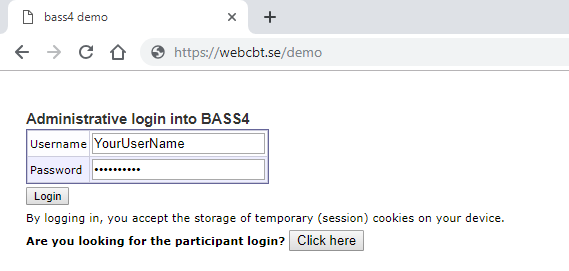
\includegraphics{images/login.png}

\hypertarget{getting-your-bearings-navigating-the-administrators-interface}{%
\chapter{Getting your bearings: Navigating the administrator's interface}\label{getting-your-bearings-navigating-the-administrators-interface}}

Now, let's turn to the administrative interface. You access this through either \url{https://webcbt.se/YourDataBase} or \url{https://bassdb.se/YourDataBase}. You will have your login credentials supplied by us, and logging in will require 2FA (two-factor authentication) through either SMS or through an authenticator app (Authy, Google Authenticator, Microsoft Authenticator).

All functionality in the BASS administration interface can be accessed from the main menu to the left of your screen.

What options are visible in the main menu depends on what privileges have been assigned to your profile. A common setup is that one administrator manages the available instruments and assessments, while several therapists manage their own participants and individual treatments. This manual is written to cover BASS in its entirety. The image below shows all available menu options, as presented to database administrators.

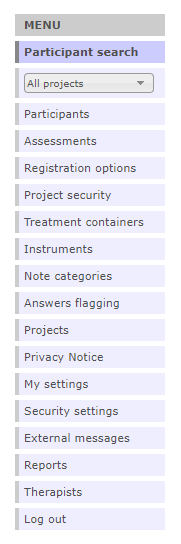
\includegraphics{images/main-menu.png}

Now, let's examine what substitutes the main menu:

\textbf{Participant Search} lets you search specific data points relevant to the participants registered in the active project. The \emph{Search} tab will show what information is searchable. See Chapter 4 for further details.

The \textbf{Project} dropdown menu lets you choose what project to view. This governs which participants and what assessments you can access. Instruments and treatments are shared between projects. To switch projects, simply use the dropdown menu.

\textbf{Participants} lets you see an overview over all the participants registered in the active project. In this overview you can see if a participant is flagged, has sent messages or reported an error, among other information. See Chapter 6 for further details.

\textbf{Assessments} is only shown if you have selected a project from the \textbf{Project} dropdown menu. Here, you can view, create and edit assessments. See Chapter 5 for further details.

\textbf{Registration options} is only shown if you have selected a project. This view lets you define the parameters of the registration procedure built into BASS, should you elect to use it. You can define what information you want participants to submit, and write detailed information about your study or treatment to be presented. You can also opt to present consent forms during the registration process. See Chapter \# for further details (under construction and will be updated).

\textbf{Project security} lets you define what security measures your project will use, such as two-factor authentication.

The \textbf{Treatment containers} view lets you view, create and edit treatments to be used within BASS. See Chapter 8 for further details.

The \textbf{Instruments} view lets you view, create, edit and delete instruments to be used within BASS. See Chapter 7 for further details.

\textbf{Note categories} lets you define custom note categories to be used to sort information on participants.

\textbf{Answers flagging} lets you set and define rules to flag specific answers or answer ranges in instruments that you want to quickly be notified about, should a participant give those answers.

The \textbf{Projects} lets your view and create projects within the database.

\textbf{Privacy notice} lets you view and edit the privacy notice(s) for the database and its projects. This is mandatory information in the EU that needs to be made available to all potential participants. If you use the built in registration procedure in BASS, this privacy notice is presented there.

\textbf{My settings} lets you view the settings of your therapist login.

\textbf{Security settings} lets you view and edit the security settings of the database, such as a general mailbox and expiry time for quick login codes. See Chapter \# for further details (under construction and will be updated).

\textbf{External messages} lets you view and edit messages which can be sent automatically to the cell phones or e-mail adresses of participants. This is, for example, notifications and reminders about active assessments.

\textbf{Reports} lets you extract reports on data collected through instruments and assessments in BASS. See Chapter \# for further details (under construction and will be updated).

\textbf{Therapists} lets you view, create and edit therapist logins in the database. See Chapter \# for further details (under construction and will be updated).

\textbf{Log out} simply logs you out of the database and ends your current session.

\hypertarget{the-intended-structure-of-a-bass-project}{%
\section{The intended structure of a BASS project}\label{the-intended-structure-of-a-bass-project}}

Now that we've familiarized ourselves with the main menu and its options, let's take a moment and look at the internal structure of BASS, and how it's set up.
As you've surely gathered by now, the foundation of BASS is the \textbf{database}. This is the foundational level upon with all other layers are applied. The next level is the \textbf{project}. You can have just one project in your database, or you can have several. Participants are placed in to projects, but may be moved from one project to another if necessary. Each project in your database will have its own registration URL, its own login URL, as well the option to use its own privacy notice.
The next level in this structure is \textbf{groups}. They can be used to group participants \emph{within} a project. This enables you do administer different sets of assessments to different groups of participants, for example. It also lets you use groups as a sorting tool in your reports.
An important note is that instruments and treatments are stored at the database level, meaning they are accessible from all projects within the database. Assessments, however, are stored at the project level and are as such not shared between projects.
And to clarify: participants and groups are also not shared between projects.

\hypertarget{setting-up-your-project}{%
\subsection{Setting up your project}\label{setting-up-your-project}}

Now, how do I set up my project? And what do I need to get started?
You can get started without setting up a project, and start by building instruments and treatments. However, it's recommended that you get into the habit of setting up your project prior to doing much else within your database. Doing so helps you stay oriented. To set up your project, simply navigate to \textbf{Projects} and click \emph{Create new project}, type a name into the box and click Save. Your new project will then be shown in a table just above the name box.

\hypertarget{groups}{%
\subsection{Groups}\label{groups}}

If you want to use groups in your project, for example to administer different cohorts, navigate to \textbf{Participants}, and to the tab labeled \textbf{Groups}. To create a group, simply type the name into the text box and click \emph{Save}. If you want to edit this name later on, you can easily do so by editing the name directly in its box and click \emph{Save} again.
If you haven't decided whether you need groups or not, you can hold off on creating groups for now. If you know you won't need groups, you can simply forgo creating any groups.

\hypertarget{settings-and-security}{%
\chapter{Settings and security}\label{settings-and-security}}

The security settings are split up between two menu options: The \textbf{Project security} and \textbf{Security settings} options, respectively. \textbf{Project security} deals with two-factor authentication for your participants in a specific project. You are given the options to provide 2FA via SMS or e-mail, or both. You can also opt to use 2FA via one of two authenticator mobile apps: Microsoft Authenticator or Google Authenticator. This option is called TOTP.
\textbf{Security settings} handles more baseline security settings for your database.

\hypertarget{security-settings-therapists}{%
\section{Security settings (therapists)}\label{security-settings-therapists}}

Here you can choose by which mean (SMS and/or e-mail) you want 2FA for therapists. Check the box or boxes for the options you want to use.
Below the 2FA options are \emph{password requirements}. Here you can specify rules for the passwords of therapist logins. You can also specify if you want mandatory password changes by typing in a number in the box labeled \emph{Monthly interval} for mandatory password change.

\hypertarget{security-settings-participants}{%
\section{Security settings (participants)}\label{security-settings-participants}}

In this table you can decide whether you want to use the quick login feature or not, as well as specify the settings for it. To allow the use of it, simply check the box labeled \emph{Allow quick login}.
In the box below, you can specify what number of days the quick login codes are valid after they've been generated (default 14 days). Be wary of allowing too long periods of time, since quick login codes does not require user names, passwords or 2FA. Before you consider using quick login codes, make sure your participants does not share e-mail accounts for cell phones with anyone else. \textbf{\emph{If another person gets hold of an active quick login code link, they will have full access to that participant login as long as that code stays active.}}
Below the duration setting, an example URL for quick login codes is shown.

\hypertarget{wait-what-are-quick-login-codes}{%
\subsection{Wait! What are quick login codes?}\label{wait-what-are-quick-login-codes}}

Quick login codes are sequences of numbers and letters that are assigned to participants. Each participant is assigned their own unique code. BASS can use these unique codes to identify the participant and log them in to their account automatically, without requiring user name, password or 2FA. This is useful if you wish to streamline the login process and lower the barriers for your participants. As mentioned above, it does pose some vital security questions however and should not be used unless you feel comfortable in that the security of your participants isn't jeopardized.

\hypertarget{lost-password-method}{%
\section{Lost password method}\label{lost-password-method}}

The options here allow you to specify how participants who report lost passwords are handled. You can choose whether to require participants to confirm their e-mail or not before they're flagged as having reported a lost password.

\hypertarget{participant-files}{%
\section{Participant files}\label{participant-files}}

This option governs whether the uploading of participant specific files is allowed. This options is provided to allow different therapists to upload for example offline paperwork as a scanned file, or a complex figure drawing. This is a solely administrative side feature, and does not allow uploading and sharing of files with the participant in question.

\hypertarget{oauth-totp-app-links-participants}{%
\section{OAuth TOTP app links (participants)}\label{oauth-totp-app-links-participants}}

This is a new feature that allows you to use authenticator apps (Google Authenticator and Microsoft Authenticator as of this writing) for two-factor authentication. This is a more secure way to use 2FA than SMS or e-mail, but requires a few more steps for the participant to activate. For participants who are less accustomed to modern technology, 2FA via SMS or e-mail may be preferrable.

\hypertarget{external-messages}{%
\chapter{External messages}\label{external-messages}}

Under this menu option, you can adjust the settings for external messages sent from BASS (SMS and e-mail), as well as type standard messages to be used for assessments and treatments.

\hypertarget{sms-settings}{%
\section{SMS settings}\label{sms-settings}}

The first box is labeled \emph{SMS sender name}, and is the name shown as the sender when a participant or therapist receives an SMS from your database.
The box below, labeled \emph{Standard SMS with quick login code}, is only relevant if you've elected to use quick login codes (see the previous chapter: Settings and Security). The message you type here will be the standard message that participants receive when their quick login codes are updated.
Nestled below that is the dropdown menu \emph{Delivery method for new message notifications to therapists}. The SMS options is as of this writing defunct, so the only valid option is ''E-post''.

\hypertarget{new-treatment-message-notification-settings}{%
\section{New treatment message notification settings}\label{new-treatment-message-notification-settings}}

Here you specify how treatment notifications will be delivered, and what the message is. You can have them delivered by SMS or e-mail, by checking the relevant radio button.
Below that, there is a box for \emph{New message email subject}. This is only relevant if you've selected the e-mail radio button above. This is the subject header for the e-mail that is sent to the participant as a notification of new treatment content.
The box labeled \emph{New message notification} is where you type the message that will be sent as an SMS or e-mail according to the settings you've specified above.

\hypertarget{sms-count-per-month}{%
\section{SMS count per month}\label{sms-count-per-month}}

This table shows you how many SMS messages have been sent from your database on a monthly basis, with a total summary at the bottom.

\hypertarget{email-settings}{%
\section{Email settings}\label{email-settings}}

Under this headline are the settings for e-mail addresses connected to your database. The first one, \emph{Sender automatic messages}, is the e-mail address that is shown when automatic e-mails are sent to participants or therapists. These are by far and large notification messages. It is set to webcbt-noreply{[}at{]}ki.se by default.
Below that is the \emph{General mailbox for database}. This e-mail address is shown to participant as the contact e-mail in case they're experiencing issues. It is also used as a fallback address in case a participant does not have a therapist assigned to them, so that they won't go unnoticed if they report a lost password or score an instrument in a manner that requires immediate attention.

\hypertarget{assessment-reminder-settings}{%
\section{Assessment reminder settings}\label{assessment-reminder-settings}}

Here you specify the settings for automatic reminders connected to assessments. You can specify at what hour you want reminders to be sent (default is 12, at noon). This works on a 24-hour basis, so you can set any whole number between 0-24.
You can also specify a time after which no reminders will be sent. This is useful if you want to spare your participant the annoyance of being reminded to complete their assessments at 23:00/11 pm.
Below these settings are two textboxes, \emph{Standard SMS assessments reminder} and \emph{Standard email assessment reminder}. In these boxes you can type standard messages for reminder notifications. If you want custom reminder messages for assessments, you can type them in the corresponding text box in the assessment editor.

\hypertarget{registration-options}{%
\chapter{Registration options}\label{registration-options}}

Under this menu option, you edit all settings related to the registration procedure. The URL for the registration is shown at the very top of the page. Underneath it is a checkbox labeled \emph{Registration possible (if closed, edit Registration closed text below)}. Check/uncheck this to enable/disable the registration.
The first table, labeled \emph{Check participant field that should be entered when registering} allows you to specify what information is required to be submitted by the participant when they register their account. These are quite self explanatory (PID number is analogous to Social Security Number, SSN).
In the larger table below that, you can edit the following:

\textbf{PID name}
This lets you specify what the PID name is. In Sweden, this is called ''personnummer'' whereas in the US it is called ''Social Security Number'', or SSN. Your country may have a different name for this, and this option lets you assign the appropriate name.

\textbf{PID format example}
By typing here, you can present an example of the format you want the PID to be submitted in, such as ''19001212-1122'' or ``YYYYMMDD-XXXX'' in the case of a Swedish example.

\textbf{Allow participants to resume registration}
Checking this box allows participants to pick up the registration process from where they left off if they close the web browser, for example. The requirement for this to function are specified, and a participant will need to use the same e-mail address and/or SMS number when they resume.

\textbf{Use BankID for identity verification}
This is a Sweden only option, that allows participants to use the e-ID solution BankID to verify their identity. This will only collect the personal information you've specified in the Check participant field that should be entered when registering.

\textbf{Allow changing BankID first and last name}
Checking this option lets participant change the first and last name collected by BankID. This is a niche option, but may be useful if a participant has submitted a name change that has not yet been updated at Skatteverket. Do note however, that first and last names may be changed by you later. Doing so is a much safer route than allowing participants to change BankID first and last name. As with the option above, any BankID-specific option is Sweden only.

\textbf{Allow duplicated BankID registrations}
This allows a participant to register multiple accounts using the same BankID. As with the options above, any BankID-specific options are Sweden only.

\textbf{Allowed calling code countries}
This setting specifies which calling code countries are allowed by this project. If you have participant from multiple countries, you have to type each relevant country code here (such as ''se'' for Sweden, ''no'' for Norway, ``dk'' for Denmark, ``fi'' for Finland, ''de'' for Germany, ''gb'' for the United Kingdom, ''us'' for the United States'', etc.) for the SMS features to function correctly.

\textbf{Registration group}
This lets you select a previously created group as the default group newly registered participant accounts are placed into. This is mandatory if you want participants to access and complete an assessment as part of their registration.
To do this, set the group as the Registration group, and active an assessment for that group under Participants, the Groups tab, sub-tab Assessments, and set a start date for the relevant assessment in the Date column.

\textbf{Automatic username}
This allows you to set an automatic username to be assigned to participant accounts, if the specified conditions are met. This can be either an E-mail address or a custom Participant ID (see below). If you do not wish to have automatic usernames, set this to none.

\textbf{Automatic password}
If you've elected to use automatic usernames, you can also use automatic passwords. Simply check the box to tell BASS to automatically generate secure passwords for participants when they register. Both usernames and passwords will be shown to the participant at the end of their registration process. If you have assigned assessments to be completed in conjunction with the registration, the username and password information will be presented to the participant before they start their assessment.

\textbf{Automatic participant id}
This lets you use automatic participant IDs, as you specify with the following options. Participant IDs useful as a anonymized way to refer to participants, and to sync data within BASS with offline data, should you have it. If you have similar codes for participant in a journal system or other records outside of BASS, you can tell BASS to use the same syntax for participant IDs.

\textbf{Automatic participant id prefix}
This lets you set a prefix for your participant IDs. This can be whatever you choose.

\textbf{Automatic participant id length}
This allows you to specify the number of digits following the prefix, or simply the number of digits if you've elected not to use prefixes. For example, if you type ''3'' into this box, the first participant to register will have the participant ID ''001'' assigned to them, the next participant will have ''002'', the next ''003'' and so on. If you use automatic prefixes, they will be added to this, such as ''Test001''.

\textbf{Require study consent}
Check this box if you wish participant to consent to being part of your study as a step of the registration process. You can edit the study consent further down on this page.

\textbf{Render markdown}
Check this box if you want BASS to render Markdown formatting. A guide on how to use Markdown can be found here: \url{https://www.markdownguide.org}

\textbf{Personal identification number validation function}
This lets you write a JavaScript function to check whether participants adhere to the PID format you've presented.

\textbf{Study information (Markdown/HTML)}
This text box lets you edit the first page shown when participant click on the registration link. The idea is that you present information on your study here, what it is about, who you are and why you are conducting the study.
As implied by the heading, you can use Markdown and/or HTML to format your text. Best practices is to choose either Markdown or HTML and stick with one of them. Markdown is simpler and quicker to learn and work with. HTML is more complex and more effortful to learn, but in return gives finer control over how content is displayed.
It is very useful to learn at least some HTML if you intend to use BASS for treatments, as the treatment modules are built with Markdown and/or HTML.
A good resource for referencing and learning HTML is found here: \url{https://www.w3schools.com}.
Below the text box is a button labeled Insert link. Clicking this box opens the file browser for your database in a separate browser tab. From here, you can set up a folder structure for document, images, sound files and videos as well as upload such files to BASS. By clicking an uploaded file, you can insert a file path into the textbox. To turn this file path into a viewable image/video or downloadable file, refer to either Markdown or HTML as appropriate. More information on this can be found under the Treatments section.

\textbf{Captcha challenge text (Markdown/HTML)}
This text box lets you edit an optional text to be shown in conjunction with the captcha challenge. The captcha challenge already includes instructions by default, but if you want to add additional information the option to do so is here.

\textbf{Study consent (Markdown)}
If you've elected to use study consent (by checking the corresponding checkbox above), this text box is where you edit the consent form. As stated under the header, users will be required to check any checkboxes you put in here (using HTML). To set up a checkbox, use the tag. For more information on checkboxes, see the following link: \url{https://www.w3schools.com/tags/att_input_type_checkbox.asp}.

\textbf{Registration finished text (Markdown/HTML)}
This textbox lets you type a text or message that is shown to participants when they have completed their registration. As stated under the header, this message is only shown if there are no assessments pending, i.e if you've set an assessment to be completed by participants in conjunction with the registration process (as describes under ''registration group''), this message will NOT be shown.

\textbf{Registration closed text (Markdown/HTML)}
As stated under the header, the message or text you type in this box will only be shown when the registration is closed, i.e if you have unchecked the \emph{Registration possible} checkbox at the top of the page.

\hypertarget{search-participants-finding-what-you-need}{%
\chapter{Search participants: Finding what you need}\label{search-participants-finding-what-you-need}}

The ``Participant search'' is located at the top of the main menu. This is where you can search for and list participants by specific variables such as groups or projects.

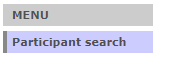
\includegraphics{images/search-participants-menu.png}

When you press ``Participant search'' you will see a view with four tabs:

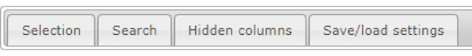
\includegraphics{images/search-participants-tab.png}

\begin{itemize}
\tightlist
\item
  Selection -- Add a filter to your search
\item
  Search -- Perform your search using text strings or other identifiers
\item
  Hidden columns -- View and show columns that are hidden
\item
  Save/load settings -- Save your recurrent searches for convenience
\end{itemize}

\hypertarget{selectionfilter}{%
\section{Selection/filter}\label{selectionfilter}}

If you press Selection, you can add a filter to your participant search.

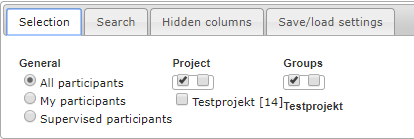
\includegraphics{images/selection-filter.png}

Here you can choose if you want to search all participants, your own participants (that you treat) or participants whose treatments you supervise.

You can also choose which project(s) or group(s) to search. The top two checkboxes can be used to quickly either mark or unmark all the below listed projects or groups. If no specific project or group is checked, all of them will be included in the search. This also means that unchecking all projects/groups won't return participants without a project/group.

\begin{quote}
\textbf{Hint:} If you want to search a specific group you should only mark that group, and not the corresponding project, as this will return all the participants belonging to the project and not only those in the group.
\end{quote}

Your chosen selection of participants is shown in the participant list below the tab.

\hypertarget{search}{%
\section{Search}\label{search}}

The actual search is done in the \textbf{Search} tab. If you previously added search filters in the Selection tab they will now be active and delimit your search.

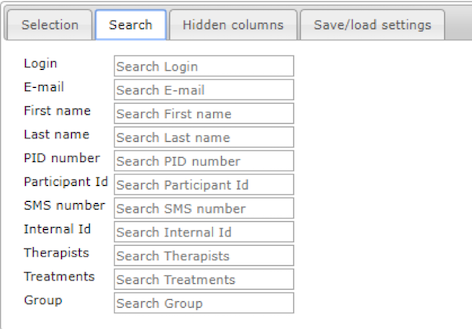
\includegraphics{images/search.png}

Here you can use many different variables to search for one or several participants. The search is executed either automatically when you leave a filled-in search box or when you hit the Enter-key on your keyboard. Your search results are shown in the participant list below the tab.

Note that there is a discrepancy when searching by numbers or by text strings:

\begin{itemize}
\item
  Searching for the number ``12'' will only show the exact hit, while adding a \% sign to the search as in ``12\%'' will return both ``12'', ``123'' and ``012''.
\item
  Searching for the text string ``my'' will return both ``My'', ``Myra'' and ``Amy''. You don't need to add any \% sign for text string searches.
\end{itemize}

To search for several participants at the same time, you add a space between each corresponding search term in the search box.

\begin{quote}
\textbf{Hint:} This is useful if you want to search for participants whose IDs are listed on different rows in an Excel-file. Just copy the ID containing rows in Excel and directly paste them into the search box in BASS and they automatically receive a space between them.
\end{quote}

\hypertarget{hide-show-and-sort-columns}{%
\section{Hide, show and sort columns}\label{hide-show-and-sort-columns}}

If you want to hide a column, you hover the mouse over the column header until a red X shows up. By pressing the X, the column will be hidden.

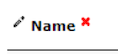
\includegraphics{images/hide-show-sort.png}

To show/unhide a column, press the ``Hidden columns'' tab. This tab shows all hidden columns as buttons. Press the button with the column you want back and it will show up in the search results again.

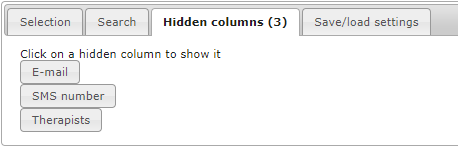
\includegraphics{images/hidden-columns.png}

Most columns can be sorted alphabetically or by number. To sort a column, press the small up/down arrows that show when you hover over the column header.

\hypertarget{column-explanations}{%
\section{Column explanations}\label{column-explanations}}

There are a number of columns showing information, status or possible actions for a participant. Some are explained in the table below.

Column

Description

Pen symbol

Edit the participant

Participant Id

A unique identifier for a participant within the study/project. ``ANX-001''

Internal Id

A unique and technical identifier for a participant within the database.

Flag symbol

Shows if the participant is flagged for something.

Message symbol

Shows if there are unread messages from the participant.

Chat symbol

(For supervised therapists)
Shows if there are unread messages from the supervisor.

Approval symbol

(For supervisors)
Shows if there are messages sent from a supervised therapist to a participant that might need approval.

Superv Mess

(For supervisors)
Total number of messages in supervisory correspondence. This is a useful way to see how much guidance was needed from the supervisor.

Last message

Last date when a participant sent a message (was active). Sort on this column and you'll find participants that are lagging behind.

Weeks

The number of weeks left of the treatment.
Treatments without end date are marked with the eternity symbol.

Module

The latest module the participant got access to. This column also shows for how many days the participant has had access to the module.

Homework

Shows if there is an unread homework sent in by the participant.

Group

Shows which group a participant belongs to. You can change the group here, but you need to save the update with the Save button below the list.

Heart symbol

By pressing the heart, you add the participant to your participants.

Trash symbol

By pressing the trash symbol, you delete the participant. Be careful as the participant and all its corresponding data then will be lost.

\hypertarget{saveload-search-settings}{%
\section{Save/load search settings}\label{saveload-search-settings}}

To save your current search settings, including both filters and search parameters, press the Save/load settings-tab. First ensure that the current search result for the settings you want to save are shown in the table below. Then write a name for your settings in the Currently loaded settings box and press ``Save as new''.

\begin{quote}
\textbf{Hint:} Be careful to not use the ``Save'' button instead, because this will overwrite any currently loaded settings including its name.
\end{quote}

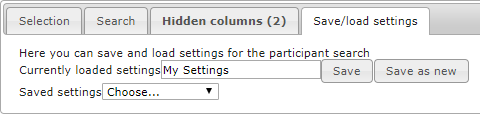
\includegraphics{images/save-load1.png}

The text ``saved!'' appears to the right of the buttons and your search is now saved and available in the dropdown below.

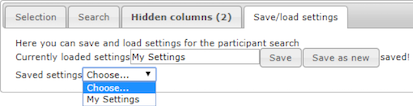
\includegraphics{images/save-load2.png}

The dropdown ``Saved settings'' is where you access all your previously saved search settings.

\begin{quote}
\textbf{Hint:} If you make a new search, the ``Currently loaded settings'' box may no longer reflect the content of the search result list below. To be sure that the list matches the settings you want to load, first select ``Choose'' in the dropdown menu and then reselect the settings you want.
\end{quote}

\hypertarget{add-new-participant-to-group-and-change-group}{%
\subsection{ADD NEW PARTICIPANT TO GROUP AND CHANGE GROUP}\label{add-new-participant-to-group-and-change-group}}

It is possible to directly create a new participant within a specific project. This function is found below the table of participants. Just choose which project you want to add the new participant to, and you will be redirected to the ``New participant''-view with this project pre-filled.

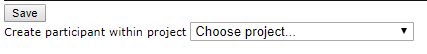
\includegraphics{images/add-new-participants.png}

It is also easy to change which group a participant belongs to. For each participant in the table, you can choose a project in the dropdown in the Group column. Don't forget to save all changes by pressing the ``Save'' button below the table afterwards.

\hypertarget{participants}{%
\chapter{Participants}\label{participants}}

The ``Participants'' view is one way to access participant information. It is very similar to the ``Participant search'' view, and it is mostly down to personal preference on which to use. You can customize ``Participant search'' to show exactly the data you want to see, while ``Participants'' is predefined and more simplistic. One important difference remains, however: the \textbf{``Groups''} tab, which only exists under ``Participants''.

Depending on which project is selected in the dropdown in the main menu, the result in the ``Participants'' view will differ. If a specific project is selected, only participants in that project wil be shown under each tab.

In ``Participants'', there are four tabs:

\begin{itemize}
\tightlist
\item
  \emph{My participants}, which shows you any participants assigned to you (as a therapist)
\item
  \emph{Supervisions}, which is similiar to ``Supervised participants''
\item
  \emph{All participants}, which shows you all participants in a project. If no project is selected, it will show all participants in the database.
\item
  \emph{Groups}, which shows you the groups created in a project, and gives you the tools to manage them.
\end{itemize}

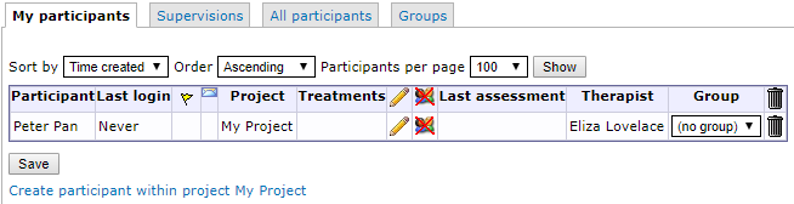
\includegraphics{images/new-images/participantsTabs.png}

\hypertarget{creating-deleting-and-editing-participants}{%
\section{Creating, deleting and editing participants}\label{creating-deleting-and-editing-participants}}

You can create new participants in two of the tabs in the Participants view; \emph{My participants} and \emph{All participants}. Participants that are created in the \emph{My participants} tab will be tagged as your participants automatically, while participants created in the \emph{All participants} tab won't be tagged.
To create a new participant, click \emph{Create participant within project {[}Project Name{]}}. Newly created participants are added at the bottom of each view.

To delete at participant, click the trash bin icon to the far right of the corresponding participant's row.

To edit a participant, click the pencil icon in the table, on the corresponding participant's row. This will take you to the ``Participant stats'' view.
If you only wish to change, or add, what group a participant belongs to, you can do so directly in the \emph{Group} column of the participant table by using the dropdown. When you've assigned a participant to a group this way, don't forget to click the ``Save'' button at the bottom of the table.

\hypertarget{the-participant-view}{%
\section{The participant view}\label{the-participant-view}}

When you create or edit a participant, the participant view is shown. To exit this view, and return to the participants table, click the ``close'' text to the right of the participant's name. If you made any changes to the participant, don't forget to save them by clicking the ``Save'' button at the bottom of the page.

There are seven tabs in this view:

\begin{itemize}
\tightlist
\item
  \emph{Participants stats}, where you can view all fundamental information on the participant
\item
  \emph{Treatments}, where you can view and manage any treatments connected to the participant
\item
  \emph{Files}, where you can upload files relevant to the participant. These files cannot be viewed by the participant, but only by therapist who have access to the participant.
\item
  \emph{External messages}, where you can manually send SMS or e-mail messages to the participant, and review the status on any previously sent external messages.
\item
  \emph{Flags}, where you can view any flags the participant might have.
\item
  \emph{Assessments}, where you can view and manage assessments for the participant. You can also activate or deactivate individually managed assessment through this view.
\item
  \emph{Graphs}, where you can see graphs on the answers the participant has given on recurring assessments.
\end{itemize}

\hypertarget{participant-stats}{%
\subsection{Participant stats}\label{participant-stats}}

This view shows information about the participant, such as ID-numbers, name, the therapist assigned to the participant (if any), any notes on the participant and more.
The \emph{Show participant log} button on the top of this view will show a log of all changes and updates done to the participant. The \emph{Show notes} button will show a log of all notes written aout the participant.
Now notes on a participant can be added by clicking the \emph{Create new note} link.

\begin{quote}
\textbf{Important note:}Prior to doing this for the first time, make sure to add at least one note category through the \textbf{Note categories}, accesssed from the main menu. Further details on this can be found in the Participant notes section in this manual.
\end{quote}

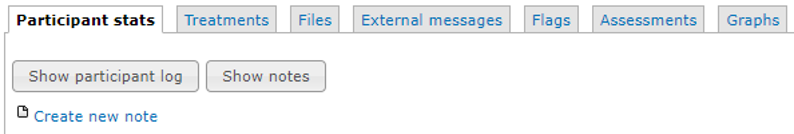
\includegraphics{images/new-images/participantStatsLogNotes.png}

The \emph{Stats} box shows data such as how many times the participant has logged in and which privacy consent was approved and when. \emph{Internal ID} is the identification number of the participant used by the database.

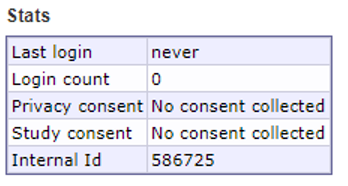
\includegraphics{images/new-images/participantsStatsSmall.png}

User information can be edited in the \emph{User information} box.

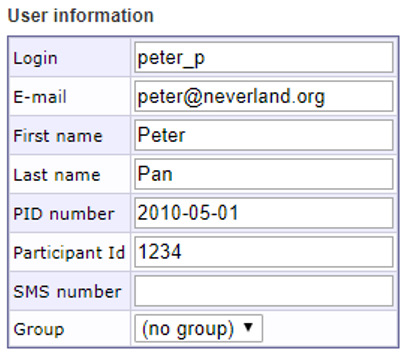
\includegraphics{images/new-images/participantInfo.png}

Existing passwords \emph{\textbf{cannot be retrieved}}, only cleared or changed. If a participant reports a lost or forgotten password, you can provide them with a link to reset and change their password by clicking the \emph{Send password link} button.
It is also possible to generate new quick login codes, and to send them by SMS, from this view.

\begin{quote}
\textbf{Important note:} Quick login settings are managed under \textbf{Security settings} in the main menu.
\end{quote}

\begin{quote}
\textbf{Important note:} \emph{Exempt from two-factor authentication} must be enabled under \textbf{Project security} in the main menu. It is only possible to exempt participants from two-factor authentication. It is mandatory for therapists.
\end{quote}

The \emph{Temporary flag text} box provides you with the possibility to flag a participant with a star icon, that will display next to their name in the participants table. You can add a comment on why you flagged the participant.

The \emph{Temporary notes} box provides you with the possibility to add a temporary note on the participant - this note is also saved in the participant log if your click the ``Save'' button.

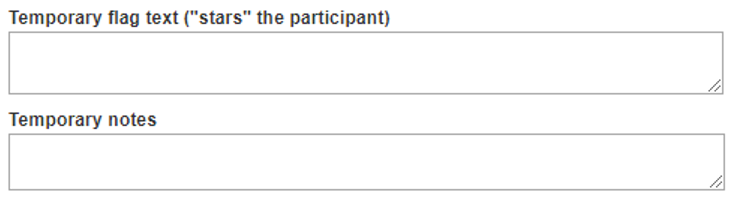
\includegraphics{images/new-images/participantTempFlagNote.png}

\emph{Assign participant to therapists} allows you to assign the participant to another, or several other, therapist(s). The number shown in brackets to the right of each therapist's name displays how many participants are already assigned to that therapist. This is useful for when you want to assign participants equally to the available therapists.
Remember to click ``Save'' to save your changes.

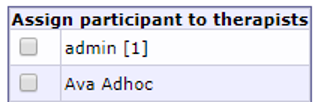
\includegraphics{images/new-images/participantTherapists.png}

You can use the dropdown menu on the bottom of the page to move the participant to another project. This will move the participant to the project of your choosing, and close the tab. If you want top view the participant again, you will need to navigate to the destination project before being able to do so.

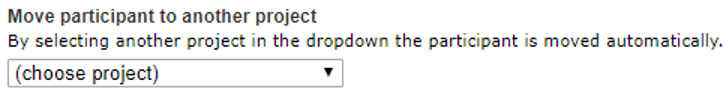
\includegraphics{images/new-images/participantMoveProject.png}

\hypertarget{participant-treatments}{%
\subsection{Participant treatments}\label{participant-treatments}}

To assign a participant to an existing treatment, go to \textbf{Participants}, \textbf{Treatments}, the \textbf{Treatment access} tab. All available treatments are listed here in the dropdown menu.

If a treatment doesn't show up in the dropdown menu, you will have to make it available via \textbf{Treatment containers} in the main menu.

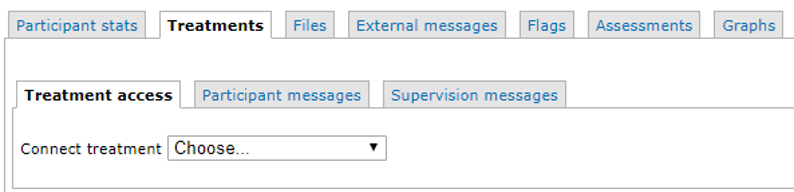
\includegraphics{images/new-images/participantTreatConnect.png}

\begin{quote}
\textbf{Important note:} While it technically is possible to assign several treatments to the same participant via the admin interface, the participate will really only be able to access \emph{\textbf{one}} of the treatments at a time.
\end{quote}

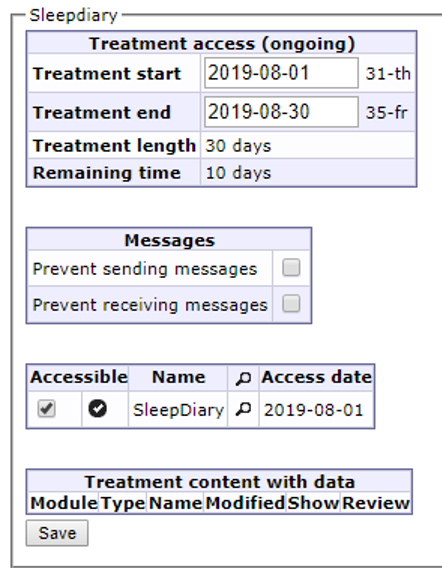
\includegraphics{images/new-images/participantTreatAccess.png}

In some studies, you may want to record how much time is spent writing messages to participants by a therapist. \emph{\textbf{More info to come}}

\hypertarget{instruments}{%
\chapter{Instruments}\label{instruments}}

In BASS, instruments are the building blocks of assessments. Under this menu option, you can view a list of all the instruments currently set up in your database, as well as Create new instrument by using the built-in editor and Import instrument from XML to import an already built instrument from another BASS database by copying its XML code. You can also edit instruments, as well as delete them.

But first, let's examine the table.

\begin{itemize}
\tightlist
\item
  To the left we have the \emph{Name} column. This simply shows the name of the instrument, as well as if it is adapted to \textbf{responsive presentation} (a small cell phone icon will be shown) and/or if it is a \textbf{clinician rated instrument} (a small, grey scroll icon will be shown). Responsive presentation means that the instrument is set up to adapt to different screen sizes, i.e desktop/laptop screens and mobile screens.
\item
  Next is the \emph{Abbreviation} column, which shows the abbreviation of the instrument (if one is specified), such as MADRS-S, HADS, PHQ-9 and so forth.
\item
  The next column is labeled \emph{Title name}, and is the title shown to participants. This can be either the proper name of the instrument, a name of your own choosing, or nothing at all.
\item
  The \emph{Id} column shows the ID the instrument is given within your database. This is useful if you want to set up Answer flags for an instrument. In such a case, you can refer to the instrument's ID rather than its name, since the ID can't be changed. As such, it is a more stable way and less vulnerable to changes.
\item
  The following column, \emph{\#Items}, displays the number of items in the instrument.
\item
  The next column, \emph{\#Completed}, displays the number of times the instrument has been completed by participants.
\item
  The \emph{\#Ass.batt. column} displays the number of Assessment batteries in which the instrument is included.
\item
  The last the columns are \emph{Edit} (the pencil icon), \emph{Copy} (the clipboard icon) and \emph{Delete} (the trash can icon).
\end{itemize}

There are two ways to create a new instrument in BASS4. Either you can copy an existing instrument, that is similar to the one you wish to create and adjust that instrument. You can also create a new instrument from scratch, using the built in tool in BASS4.

\hypertarget{copy-an-instrument}{%
\section{Copy an instrument}\label{copy-an-instrument}}

To copy an instrument, follow these steps:
1) Navigate to \textbf{Instruments} in the main menu to the left. Here you can view all instruments currently available in your database.
2) On the far right of the instrument you wish to copy, next to the trash can icon, is an icon resembling two documents. If you hover with the mouse pointer over this icon, it will say ``Copy instrument''. Clicking on this icon will create a copy of the instrument, called ``Copy of {[}Instrument{]}''.
3) Open the instrument you just created by clicking the pencil icon to the right on the instrument row. If you hover the mouse pointer over the pencil icon, it will display the tooltip ``Edit instrument''. Clicking the pencil icon will show the instrument editor. The ``Creating a new instrument'' section explains how this editor works.
4) Prior to editing the instrument, it's good practice to open a separate window or browser tab by using the \textbf{Preview-function}. This function is located under the Preview-tab, and opened by clicking the ``Open preview in Clojure app'' hyperlink. By default, a new tab will open where the instrument will be displayed in its formatted layout. It's a good idea to have this tab opened while editing the instrument in the instrument editor, and switching back and forth between the browser tabs to see your updates displayed in the Preview.

\hypertarget{creating-a-new-instrument}{%
\section{Creating a new instrument}\label{creating-a-new-instrument}}

To begin creating a new instrument, navigate to \textbf{Instruments} in the main menu on the left. This will open up a table view showing you all the instruments currently available in your database. On the bottom of the table, there is a hyperlink with the text ``Create new instrument''. Clicking this hyperlink will take you to the \textbf{General} view of the instrument editor, as shown in picture 1 below. The tabs named \textbf{Edit}, \textbf{Preview}, \textbf{Scoring Formula} and \textbf{Export} are also displayed.

\hypertarget{the-general-tab}{%
\subsection{The General Tab}\label{the-general-tab}}

This tab is where you can change the \textbf{Name} of the instrument, its \textbf{Abbreviation} (both of which are only show in the administrator's view), as well as the \textbf{Title name} (which is the title presented to the participants).
For example, this could be \textbf{Audit} in all three cases, as show in picture 1 below.

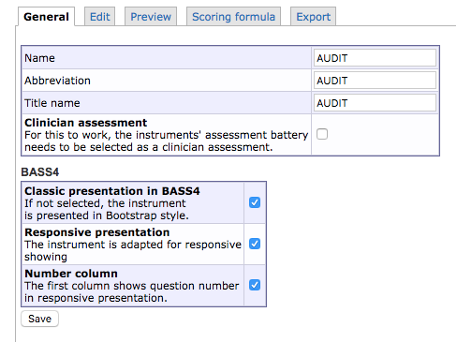
\includegraphics{images/new-images/InstrumentsGeneral1.png}
\textbf{Picture 1}

If the instrument you are creating is supposed to be filled out by a clinician, you check the box called \textbf{Clinician assessment}.

\hypertarget{the-bass4-table}{%
\subsubsection{The BASS4 Table}\label{the-bass4-table}}

This table contains three options that influence the presentation of your instrument.
\textbf{Classic presentation in BASS4} governs whether your instrument is shown in a classic layout, i.e somewhat smaller font size, or a more modern layout with a somewhat larger font size (16 pixels).
\textbf{Responsive presentation} governs whether or not your instrument is adjusted automatically according to the size of the screen it is viewed on (i.e mobile or PC/Mac). This mainly affects \emph{Question} items, where answers ordered by cell will require additional steps be taken in order to display correctly.Instructions on how to do this are found under the ``Edit'' section.
Answers ordered by line break will automatically display correctly both on mobile and PC/Mac with this option checked.
Leaving this box unchecked will cause the instrument to display its PC/Mac layout regardless of which screen it is viewed on. It will not adjust to mobile screens.
\textbf{Number column} governs whether or not the first column of the instrument is assigned to the display of question numbers in responsive presentation.

When you've entered the information, click \textbf{save}.

\hypertarget{the-preview-tab}{%
\subsection{The Preview Tab}\label{the-preview-tab}}

In this tab, you can view the instrument with it's final visual design applied (the final visual design is applied automatically by BASS) by clicking the hyperlink named ``Open preview in Clojure app''.
By default, a new tab will open, in which the instrument will be displayed with its final visual design applied. It's a good idea to have this tab opened while editing the instrument in the instrument editor, and switching back and forth between the browser tabs to see your updates displayed in the Preview.

\hypertarget{the-edit-tab}{%
\subsection{The Edit Tab}\label{the-edit-tab}}

This tab is where you create, or build, your new instrument. This is also where you adjust any instrument you've copied or want to edit. This is mainly done through adding, editing or deleting content in the form.
To begin, start by creating and defining a \textbf{table definition}

\textbf{Add table definition}
By default, the first table definition is already created. However, it has not been defined, and thus you need to define it before proceeding to adding additional items and elements to your instrument. To do this, click the ``Edit'' text in the \textbf{Table definition} box. This opens up the editor for this specific item (in this case a table definition).
One thing to note before starting to assign \textbf{Cell width} is that the total width of your instrument is fixed to 700 pixels on PC/Mac. As such, you will have to stay within those confines when defining your table definition.
If responsive presentation is used, the instrument width will adapt to a mobile screen size where applicable.

A table definition provides a layout framework for every item below it, up until the next table definition (if there is one).

A good practice is to allow the first column to take up 30 pixels of screen space. This is done by typing 30 into the first box of the \textbf{Cell width} column. If you so wish, you can justify the text of a box to be either left aligned, centered, or right aligned by choosing the corresponding option in the box's dropdown menu in the \textbf{Justify} column.
The second cell is most often reserved to the text of a question, and can be set to the desired width by typing it into the box.
Typing a * into the box makes its cell flexible, causing it to fill any left over width not claimed by the other cells in the table definition. If multiple cells are given a flexible width by typing * in their cell width boxes, they will share the left over width evenly.
The third through 16th cell is usually utlized for answers to a question item, when ordered by \textbf{Cell} (horizontally) and can be given any desired width. However, remember that width is limited if you are ordering answers by \textbf{cell}, and that long words in an answer may clip into eachother if the allocated space is too small.
Ordering answers by \textbf{line break} organizes them in a vertical structure, and as such they do not suffer this limitation. If you plan to order your answers by \textbf{line break} you only need to fill in the boxes for cell 1 and 2 in your table definition that governs the layout for the question items that utilizes \textbf{line break}

\textbf{Add information}
Usually a form starts with information on how to fill it out, and as such you want to add that information before you add your questions. To do this, click ``Add new {[}Free text{]}'' and type the information ionto the ``Free text'' box.

In ``Free text'' you type regular HTML or regular text input. You can find some basic HTML tags in the appendix of this manual, with links to more thorough resources listed as well.
In ``Layout-string'', you type {[}T{]}, which instructs BASS to render the text in the ``Free text'' box. Then press save.

\begin{quote}
\textbf{Hint:} If you want to have a line above or below your text, to act as a separator, you can type in 1 in the ``Border-width upper'' or ``Border-width lower'', respectively.
\end{quote}

\textbf{Adding questions}
Depending on what questions you would like to add, you go about adding them in different ways. We will adress the most common type of question below.

\textbf{Adding multiple-choice questions}
By follow the instructions below, your end result will look similar to this:

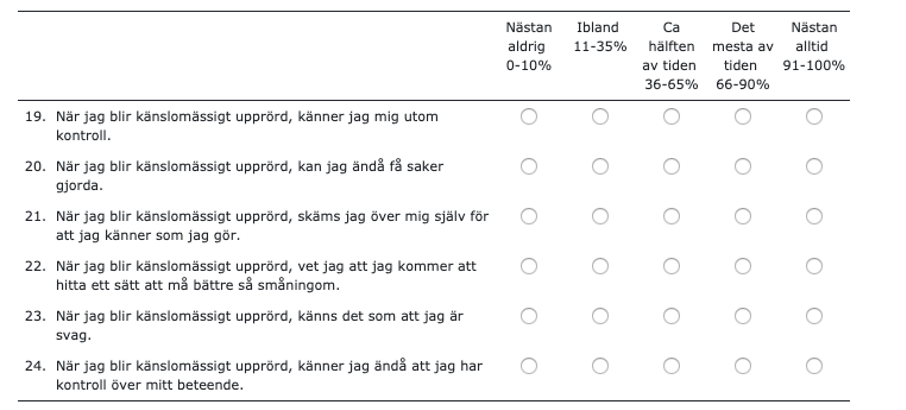
\includegraphics{images/new-images/multiplechoiceQ.png}

First, you will need to add a new ``free text''. To do this, click ``\textbf{Add new {[}Free text{]}}''. Then type in the options that are needed for the questions you want to add. For example, if you have five options to your question, you type it in like in picture 4 picture below.
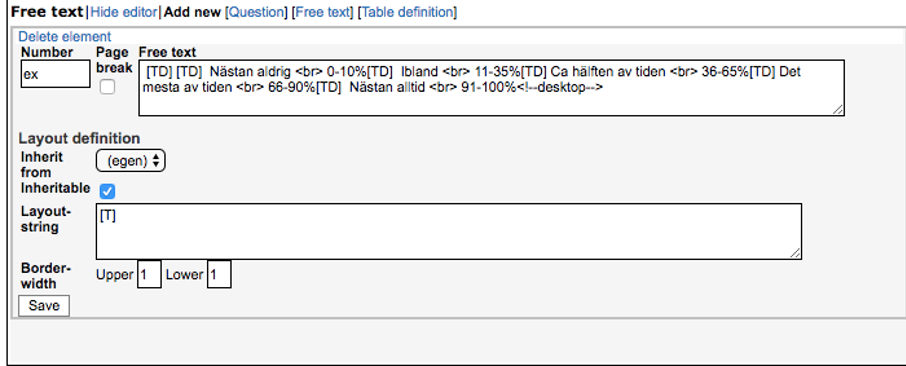
\includegraphics{images/new-images/multiplechoiceFreeText.png}
\textbf{Picture 4}

If you have more options, you add them by typing ``{[}TD{]} option 6'', before the HTML tag \texttt{\textless{}!-\/-desktop-\/-\textgreater{}}. If you have less options, you delete the superfluous {[}TD{]} with accompanying text. The reason for the twin {[}TD{]}{[}TD{]} in the beginning is to make empty space for the question you're adding later. The reason for the single {[}TD{]} between the options is to separate the options.

\begin{quote}
\textbf{Hint:} \texttt{\textless{}br\textgreater{}} is HTML and means that the rest of the text starts on a new row, i.e it implements a line break. If you want to have numbers on one row and the text under, you can add two tags in between. If it's all supposed to be on the same row, you can omit including any \texttt{\textless{}br\textgreater{}} tags.
\end{quote}

Like in the ``Free text'' example, you type {[}T{]} in ``Layout-string'' to instruct BASS to render the text. Then decide whether or not you want borders above or below the text by typing in a numerical value in ``Border-width upper'' or ``Border-width lower'', respectively. Then click ``Save''.

Below the created ``free text'', you now click ``\textbf{Add new {[}question{]}}''. In the number box, you type in the number you want to assign to the question. In the ``Question''-box you type in the question or statement.

By using the tools in the ``Answer definition'' section, you can define what type of answer you want. By default, ``\textbf{Radio buttons}'' is selected as the ``Answer type''. If you want multiple choice, you change the ``Answer type'' to ``\textbf{Checkboxes}''.
You can then fill out the different options under ``label'' (in this example you would use the same options you typed in ``free text'') and give them unique values under ``value'', see picture 5 below. The values are used to calculate the result with a scoring formula later on.

\begin{quote}
\textbf{Important note:} The values for each answer option in a question \emph{have} to be unique. If to answer options are supposed to have the same value, this is corrected for later on in the scoring formula.
\end{quote}

When you've filled in your answer options and their unique values, you can choose ``Cell'' under the ``Separator''-dropdown. In ``Layout definition'' you type in the following: \textbf{{[}N{]}.{[}TD{]}{[}Q{]}{[}TD{]}{[}X{]}}. This defines the layout for the question within the framework provided by your table definition. When this is done, click ``Save''.

\begin{quote}
\textbf{HELP! What does {[}N{]}.{[}TD{]}{[}Q{]}{[}TD{]}{[}X{]} mean?}
\end{quote}

\begin{quote}
\begin{itemize}
\tightlist
\item
  {[}N{]} Renders the number of the question in a cell. The period simply puts a period after the rendered number.
\item
  {[}TD{]} Creates an empty cell
\item
  {[}Q{]} Renders the text of the ``Question'' box in a cell
\item
  {[}X{]} Renders the answer options in a cell
\end{itemize}
\end{quote}

The input in the ``layout definition'' box is read from left to right, and is applied in the same order. In the layout above {[}N{]} is rendered in the first cell, {[}TD{]} creates a space, {[}Q{]} is rendered in the second cell and {[}X{]} is rendered in the third through seventh cell.

\begin{quote}
\textbf{Hint:} Make a habit of going back to your Preview page to see what your form looks like. This lets you correct mistakes and make adjustments as you go along.
\end{quote}

\begin{quote}
\textbf{Hint:} You can read about ``optional'', ``inheritable'', ``jump'', and ``specification text'' under ``Extra information''.
\end{quote}

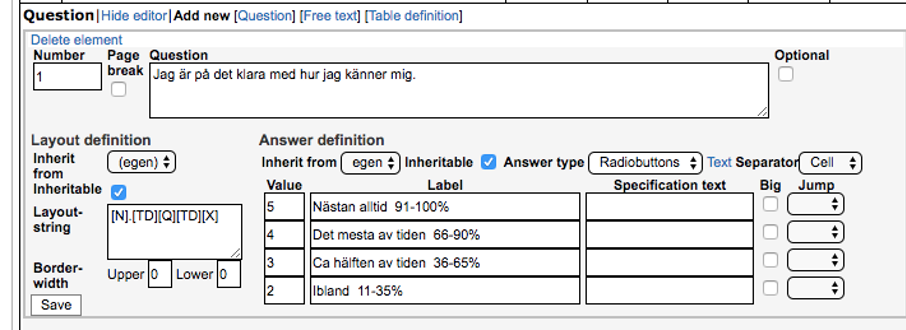
\includegraphics{images/new-images/multiplechoiceQuestion.png}
\textbf{Picture 5}

\textbf{Adding a text-answer question}
To add a question with a text answer, click ``\textbf{Add new {[}question{]}}''. Follow the same procedure as detailed above, by typing the number you want to assign to the question in the number box, and typing your question or statement into the question-box. Under ``Answer definition'', choose what type of answer you want, either ``short free text'' or ``long free text''. In ``Layour-string'', type in \textbf{{[}N{]}.{[}TD{]}{[}Q{]}{[}X{]}}.

\textbf{Having the multiple-choice answer options listed vertically instead of horizontally}
If you would rather have your answer options listed vertically below your question, you type the question in a Free text. To do this, click ``\textbf{Add new {[}Free text{]}}''. Then type the question into the free text box, and type \textbf{{[}T{]}} into the layout-string box.
Below the ``free text'' you just created, click ``\textbf{Add new {[}question{]}}''. In the number box, assign the number you wish your question to have. Leave the ``question''-box empty.
Proceed to fill out the ``Answer definition'', and type in your answer options and their unique values. Then, choose ``Line break'' in the Separator-dropdown.

\hypertarget{extra-information}{%
\subsection{Extra information}\label{extra-information}}

\textbf{Optional questions}
If the question is not mandatory, you can tell BASS to treat it as such by checking the ``optional''-box, in the upper right corner of the question-editor window. This enables a participant to complete the form without submitting an answer to that specific question.

\textbf{Page break}
If you want a question to appear on a new page, you can tell BASS to divide your form into pages by checking the ``page break''-box in the upper left corner of an editing window. By checking this box, the item for which you check it will be the first item to display on the new page. The following items will show on the new page.

\textbf{Using the jump function}
If you want an answer option to skip a participant ahead in your form, for example if a subset of questions isn't relevant if a particular answer option is selected, you can do so by using the ``jump''-function. You find this function to the right of each answer option. Open the dropdown, and select the item you wish that answer option to skip ahead to.

\textbf{Re-use layout and options}
If you have multiple questions that use the same layout and/or the same options, you can check the ``inheritable''-boxes for ``layout-string'' and/or ``answer options''. This enables the settings of one question to be inherited by another. In the editing window of the questions you wish to be inheriting settings, use the ``Inherit from''-dropdown and choose the question you want them to inherit from.

\textbf{Adding more questions}
\emph{Adding a multiple-choice question that have the same options as the previous question}.
If you want to add more questions with the same options as the previous question you just created, click ``\textbf{Add new {[}question{]}}'' and fill out the new question like you did the previous one.

\begin{quote}
\textbf{Hint:} Don't forget that you can use the ``inherit''-function. Read more about this function in the ``Extra information''-section, ``Re-use layout and options''.
\end{quote}

\emph{Adding a multiple-choice question that do not have the same options as the previous question}.
If your next question has a different set of answer options than the previous one, but the same number of answer options, you add a new free text and write the options like previously instructed, and then add the new question.

If your next question has a different \textbf{number} of options as the previous question, you need to add a new ``table definition'' that provides a new layout framework that fits the structure of the new question. Then proceed to add the new free text and question as previously instructed.

\emph{Adding a text-answer question}.
Create a new question by clicking ``\textbf{Add new {[}question{]}}'' and fill it out like previously instructed.

\hypertarget{scoring-formula}{%
\section{Scoring formula}\label{scoring-formula}}

In the \textbf{Scoring formula} tab, you can define formulas that calculate the scores from the different items in your instrument. You refer to specific items in your instrument by using the \texttt{@\#} identifier, i.e \texttt{@1} refers to question 1, \texttt{@2} refers to question 2, and so on.
Should you leave the scoring formula blank, you will still get all value readouts from your instrument. The scoring formula is meant to help with calculating different scores that are relevant to your instrument.

\begin{quote}
\textbf{Defining a calculation:} \texttt{sum\ =\ @1\ +\ @2\ +\ @3\ +\ @4\ +\ @5}
\texttt{\#sums\ sum}
\end{quote}

If you want to calculate several sums or products, you define each score (\texttt{sum}) by giving it a number.

\begin{quote}
\textbf{Adding several scores:} \texttt{sum1\ =\ @1\ +\ @2\ +\ @3}\texttt{sum2\ =\ @4\ +\ @5\ +\ @6}\texttt{sum3\ =\ @7\ +\ @8\ +\ @9}\texttt{\#sums\ sum1,\ sum2,\ sum3}
\end{quote}

\begin{quote}
\textbf{Multiplying several scores:} \texttt{sum1\ =\ (@1\ *\ @2)\ +\ (@3\ *\ @4)} \texttt{sum2\ =\ (@5\ *\ @6)\ +\ (@7\ *\ @8)} \texttt{\#sums\ sum1,\ sum2}
\end{quote}

You can also calculate the mean of a score, by dividing the number of questions included.

\begin{quote}
\textbf{Calculating the mean of a score:} \texttt{sum1\ =\ @1\ +\ @2\ +\ @3\ +\ @4\ +\ @5} \texttt{mean1\ =\ @1\ +\ @2\ +\ @3\ +\ @4\ +\ @5\ /\ 5}\texttt{\#sums\ sum1,\ mean1}
\end{quote}

Just as you can calculate several sums and products, you can also calculate several means.

\begin{quote}
\textbf{Calculating several means:} \texttt{mean1\ =\ (@1\ +\ @2\ +\ @3)\ /\ 3} \texttt{mean2\ =\ (@4\ +\ @5)\ /\ 2} \texttt{mean3\ =\ (@6\ +\ @7\ +\ @8\ +\ @9)\ /\ 4} \texttt{\#sums\ mean1,\ mean2,\ mean3}
\end{quote}

\hypertarget{export}{%
\section{Export}\label{export}}

The export tab lets you copy the XML code of an instrument, to enable exporting to another database or another program that can accept instruments/forms in XML format.

\hypertarget{assessments}{%
\chapter{Assessments}\label{assessments}}

Assessments are accessed from the ``Assessments'' option in the main menu. Note that you first have to choose a project in the dropdown in the main menu to make the Assessments option for that project visible. When you press ``Assessments'' you will see a view showing the existing assessments of the chosen project. All assessments that are listed in this view can be manually sorted with the upwards pointing arrow symbols to the right of each assessment name.

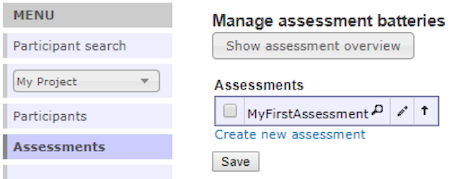
\includegraphics{images/assessement.png}

You can show or hide the expanded overview by pressing the Show assessments overview-button. Here you can get a quick review of all the included assessments and their corresponding attributes.

\textbf{Hint:} Among other things, the assessment overview shows the order of each instrument in all assessments. This is a good place to ensure that the instrument order is kept from one assessment to another throughout the project. It also enables you to easily see if you somewhere have missed to include an instrument that should appear in several, similar assessments.

\hypertarget{create-or-edit-assessments}{%
\section{Create or edit assessments}\label{create-or-edit-assessments}}

Add a new assessment to your project by pressing ``Create new assessment'' at the bottom of the Assessment view. To instead edit an existing assessment, press the pencil symbol to the right of the name of the assessment you want to edit. This opens up the assessment panel where you can set a number of variables that define the assessment:

\hypertarget{name}{%
\subsection{Name}\label{name}}

Here you can fill in a name for your assessment, for example \textbf{\emph{Screening}}.

\hypertarget{labelcustom-label}{%
\subsection{Label/Custom label}\label{labelcustom-label}}

You can either select one of the predefined labels in the drop-down, or write your own label in the Custom label textbox. Adding a custom label will surpass any predefined label that is selected from the drop-down. Note that the assessment label will be visible in reports when you export your data.

\begin{quote}
\textbf{Hint:} By selecting Weekly-assessment or Point-assessment some stats for Repetition (below) are preset.
\end{quote}

\hypertarget{managed}{%
\subsection{Managed}\label{managed}}

This option sets whether data-gathering is managed individually or in groups.

\begin{quote}
\textbf{Hint:} If you have different cohorts, you may want to choose In group. Screening assessments are usually managed In group and these can be activated or deactivated for a certain group and date under Participants -\textgreater{} Groups -\textgreater{} screening group name -\textgreater{} Show -\textgreater{} Assessments.
\end{quote}

\begin{quote}
\textbf{Hint:} If your participants start their treatments at different times, you usually choose Individually. The Individually option is also more flexible for long-term studies spanning over months when participants go for vacation and need some individual adjustment to the timing of assessments.
\end{quote}

\hypertarget{repitition}{%
\subsection{Repitition}\label{repitition}}

The Repetition option sets if the assessment is to be done once or repeatedly, and if so at what intervals and for how many times.

Assessments with the predefined label ``Weekly'' have repetition set to Weekly and the interval to 7 days.

Assessments with the label ``Point-assessment'' have repetition set to Manual. This means that the next assessment can be set manually to occur at an arbitrary date, independent of the time of the previous assessment. This is useful for assessments that are triggered by irregular events, for example a major flair of symptoms.

\hypertarget{time-limit}{%
\subsection{Time limit}\label{time-limit}}

Here you can set if participants have to fill out the assessment within a certain time limit.

\begin{quote}
\textbf{Important note:} Setting a time limit for an assessment is extremely important to prevent the results being mixed up with those from similar, subsequent assessments. For example, if an ongoing POST assessment is still accessible when the FOLLOW UP assessment is activated, the results of any of them is duplicated to the other. This results in data reports where no change seems to have occurred between the assessments.
\end{quote}

An assessment with the time limit of 7 days that starts on a Monday will be available for the rest of that week but not for the next.

\begin{quote}
\textbf{Hint:} Keeping the time limit short, or shorter than the repetition interval, has the effect that participants fill in correct data corresponding to the set time-frame, but sometimes will miss the window when they can report. This is useful in assessments where accurate and time-dependent data is more important than full attendance.
\end{quote}

\hypertarget{dependence}{%
\subsection{Dependence}\label{dependence}}

The Dependence option sets when the assessment is to be activated, in relation to the date of a previous assessment. The relationship is kept even if you change the date of the previous assessment.

Date offset from is where you select the previous assessment from which the date/delay is to be calculated.

\begin{quote}
\textbf{Note:} Setting Date offset from a reccurring assessment (i.e.~WEEKLY) will count the delay from the date of the last assessment and not the first. If this is not what you want, consider creating a dummy assessment without instruments to hold the start/dependence date.
\end{quote}

Checking Dynamic means that the delay is calculated from the time when the previous assessment was completed instead of the time when it was scheduled. Note that this setting only can be done on individually managed assessments.

Delay is the number of days to wait before activation.

\begin{quote}
\textbf{Hint:} If you can't see the calculated date of your assessment in the view under Participants -\textgreater{} Groups -\textgreater{} group name -\textgreater{} Show -\textgreater{} Assessments, try to set the date of the previous interrelated assessment again and press the Save button.
\end{quote}

\hypertarget{clinician-rated}{%
\subsection{Clinician rated}\label{clinician-rated}}

This option hides all instruments in the assessment for participants and instead enable clinicians to fill in the associated `clinician rated' instruments via the administration interface.

This setting allows a clinician to fill in the instrument(s) for a specific patient via Main menu -\textgreater{} Participants -\textgreater{} Groups -\textgreater{} specific group -\textgreater{} specific participant -\textgreater{} Assessments -\textgreater{} specific assessment -\textgreater{} specific instrument -\textgreater{} pen on document symbol

\begin{quote}
\textbf{Note:} Clinician rated instruments should not be added to self-assessments. Clinician-rated instruments are hidden for participants which makes it impossible for the participant to complete an assessment containing such an instrument.
\end{quote}

\begin{quote}
\textbf{Hint:} Clinician rated assessments won't send automatic reminders. An option is to use flags instead to mark undone tasks.
\end{quote}

\hypertarget{randomize-instrument-order}{%
\subsection{Randomize instrument order}\label{randomize-instrument-order}}

With this option you set the order of the included instruments to be randomized. If not set, the order in which the instruments appear in the assessment will be the same as the order they are presented in the box Assessment Instruments shown to the right.

\hypertarget{welcomethank-you-text}{%
\subsection{Welcome/Thank you text}\label{welcomethank-you-text}}

Here you write messages formatted in either Markdown or HTML that you want to show to participants before (welcome) and after (thank you) they fill in the assessment.

\hypertarget{concurrent-and-merged-assessments}{%
\subsection{Concurrent and merged assessments}\label{concurrent-and-merged-assessments}}

With this option you can set the order in which coinciding assessments appear to participants.

If two or more assessments can coincide, you may want to set in which order they appear to participants. This also affects the order of the Welcome/Thank you-messages. The assessment with the lowest number has the highest priority and is shown first. The other assessments and their Welcome/Thank you-messages will follow corresponding to their respective priority order.

The \textbf{\emph{Merge assessment\ldots{}}} box sets if an assessment is to be integrated as a part of (after the Welcome text and before the Thank you text) a coinciding, higher-prioritized assessment. Setting this option means that the current Welcome/Thank You-messages are not shown at all on coincidence, but only when the assessment occurs alone or simultaneously as lower-prioritized assessments.

The \textbf{\emph{If merged}} -- Show\ldots{} box sets if Welcome/Thank you-messages are to be shown even on coincidence as per the Merge assessment setting above. Note that it can be tricky to write messages that work both standalone and together with/as part of other assessment messages.

\hypertarget{automatic-reminders}{%
\subsection{Automatic reminders}\label{automatic-reminders}}

This option sets notes or reminders to automatically be sent to participants on certain events. The basic functionality is that a note is sent the same day as an assessment becomes available. With the check boxes you can choose which media to use, mobile text messages (SMS) and/or email.

\emph{Create new quick login} needs to be checked if quick logins are to be sent with the reminders.

\begin{quote}
\textbf{Hint:} Remember that you also need to activate quick login under Security Settings in the Main menu to enable this function.
You can also add reminders to participants who are late with filling in their assessments.
\end{quote}

\begin{quote}
\textbf{Note:} It is not possible to only send remainders to participants that are late with filling in their assessments, you always need to activate availability notes too (by checking either of the sms/email boxes) for this extra functionality to be enabled.
\end{quote}

\emph{Remind interval} is the delay upon which reminders are sent to late participants, counted as days after the assessment became available.

\emph{Max number of reminders} sets how many reminders can be sent out to the participant, with the previously mentioned time interval. This setting needs to be at least 1 for any reminder to be sent.

\begin{quote}
\textbf{Hint:} If you want additional reminders to be sent, increase the number in this box instead of rescheduling the assessment (see below)
\end{quote}

\begin{quote}
\textbf{Note:} Postponing an assessment that has automatic reminders to the future will neither make any new availability notes to be sent out, nor make any additional reminders to be sent out (because BASS counts the number of sent reminders independently of assessment date). Rescheduling an assessment that has automatic reminders to the past will disable the availability note (because the first day of availability has passed) and eventually disable reminders if the remind interval for them has passed.
\end{quote}

\emph{Use standard text for e-mail/SMS} -- Sets the content of reminders/notes to be sent to a predefined standard text. The current standard texts are shown below the checkbox.

\begin{quote}
\textbf{Hint:} The standard texts for reminders and notifications can be edited via Main menu -\textgreater{} External messages.
\end{quote}

It is also possible to set a \emph{Custom notifications/reminders} text in the corresponding textbox. This text is shared between emails and SMS. The \emph{Subject for activation} emails and SMS can however differ and are set in the two bottom textboxes. Custom notifications/reminders can be up to around 150 characters long.

\hypertarget{participant-flagging}{%
\subsection{Participant flagging}\label{participant-flagging}}

This option sets flags to be shown for therapists on certain, participant-specific events.

\emph{Flag participant when assessment becomes activated} raises a flag for participants at the activation of the assessment.

\emph{Flag late participants} raises a flag for participants that haven't filled in an assessment within a certain number of days after it became available. You can set the number of days to wait before flagging in the box labeled \emph{Days until participant is flagged late.} If an assessment is late, a flag will immediately be shown on the participant in question in the overview pane under \textbf{Participants}.

\hypertarget{copy-assessment}{%
\section{Copy assessment}\label{copy-assessment}}

You can create a copy of an assessment and save it to the same project before editing it. This functionality makes it quick and easy to create several similar assessments that occur at different time points within your project.

It is also possible to mark several or even all assessments of a project and copy them to another project, thus creating two similar projects.

To copy assessments in the Assessment view, check the boxes of the assessments you want to duplicate. This makes the dropdown menu Copy selected assessments to\ldots{} appear below the assessment list. From the dropdown you can select the project where you want to paste the assessment. If it is the current project, the copy-pasted assessments will appear at the bottom of the list with the prefix COPY.

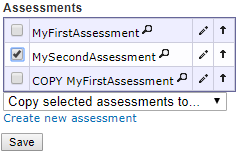
\includegraphics{images/copy-assessment.png}

\hypertarget{dummy-assessments---some-scheduling-tricks}{%
\section{Dummy assessments - some scheduling tricks}\label{dummy-assessments---some-scheduling-tricks}}

Empty assessments that doesn't contain any instruments can be used as timers to schedule administrative activities.

\textbf{Example 1, Scheduling automatic events:} A single, empty assessment can be created to hold the time point from which other assessments are scheduled to automatically become available. This circumvents the issue when a ``real'' but reoccurring assessment can't be used as starting date for a timetable.

\textbf{Example 2, Scheduling manual actions:} An empty assessment can also be used together with flagging to prompt a certain action from the therapist. This is useful when something needs to be manually sent or done by the therapist a certain number of days into treatment while participants have individual treatment start dates. The trick is achieved by creating an empty assessment (i.e.~FLAG FOR SENDING DEVICE) that is dependent on a previous assessment (i.e.~FIRST ASSESSMENT) and activated with a chosen delay (i.e.~63 days after). By checking the box Flag participant when assessment becomes activated, the therapist will see individually occurring flags on participants whenever it is time for them to receive the attention/service from the therapist. Since the assessment doesn't contain any instruments, only the therapist will get a notice (flag).

\textbf{Example 3, Scheduling text messages (SMS):} An empty assessment that is managed In group and linked to a text message can be used to schedule an independent reminder to all participants (i.e. ``Happy New Year! If you find it hard to keep to your new lifestyle during events like this, log in and re-read the advice in module 3''). An empty assessment can also be created to remind a single individual that hasn't done so for a while to log in.

\hypertarget{assessment-instruments}{%
\section{Assessment instruments}\label{assessment-instruments}}

All available instruments are listed in the right panel of the Assessment view. To include an instrument, check the box to the left of its name and then press the \emph{Save} button. The number shown between the brackets to the right of each instrument name shows how many questions the instrument contains. The \emph{Total number of items} top row shows the current total sum of questions in the assessment.

The order in which the instruments appear in the assessment will be the same as the order they are presented in the box Assessment Instruments shown to the right. You can change the order of an instrument listed in the box by pressing the upward arrow to the left of the instrument name.

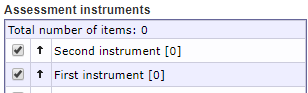
\includegraphics{images/assessment-instrument.png}

\begin{quote}
\textbf{Hint:} If you can't see any/all arrows, first select the instruments you want to include and press Save. Then change the order of the instruments and press Save again
\end{quote}

\hypertarget{create-new-treatment}{%
\chapter{Create new treatment}\label{create-new-treatment}}

BASS is designed to allow you to conduct mental healthcare and psychological studies through online channels. The main feature to achieve this in BASS, is the treatment.
A treatment is built by combining \emph{treatment modules} into sections. A module is in essence a website, contained within the framework that BASS provides. This allows you the flexibility to build your treatment according to your organization's needs and wishes.

Treatments are accessed by the \textbf{Treatment containers} option in the main menu.

The first thing you will see in this view is a table showing you all the existing treatment containers in the current project. If no treatment containers have been created, the table will be empty.
You can edit existing treatment containers by clicking the \emph{Edit} link in the column to the right.
To create new treatment containers, click the \emph{Create new treatment container} link below the table.

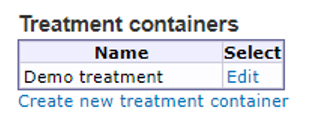
\includegraphics{images/new-images/treatmentContainers.png}

\begin{quote}
\textbf{Important note:} \emph{Treatment containers} in BASS are frameworks that contain all the other components that make up a treatment, such as treatment modules.
\end{quote}

\hypertarget{a-typical-treatment-structure}{%
\section{A typical treatment structure}\label{a-typical-treatment-structure}}

A \textbf{treatment container} is the abstract structure that holds all the content of a treatment or treatment series. A typical \textbf{treatment} is built up by several modules, often arranged in a specific order. A typical \textbf{module} consits of:

\begin{itemize}
\tightlist
\item
  One \emph{module text}
\item
  (0 - several) \emph{worksheets}
\item
  One \emph{homework}
\end{itemize}

Whenever you create a new treatment, it is advisable to plan the structure from the beginning, so as to get a sense of both the magnitude of the sub-content and the flow of the treatment.

\hypertarget{creating-a-treatment-container}{%
\section{Creating a treatment container}\label{creating-a-treatment-container}}

In the \textbf{Treatment containers} view, click the \emph{Create new treatment container} link below the table. This opens the editing view of the new treatment container. You can close the container by clicking \emph{Close} at the top to return to the table listing all existing treatment containers. Don't forget to save any changes first, by clicking the \emph{Save} button.

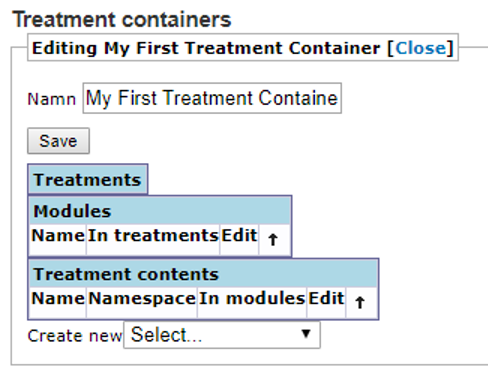
\includegraphics{images/new-images/treatmentsEditContainer.png}

Give your treatment container a name in the \emph{Name} box, and save it.
You can now add treatments, modules and specific contents such as texts, worksheets and homeworks to your treatment container, by using the dropdown menu at the bottom of the page.

\hypertarget{creating-a-treatment}{%
\section{Creating a treatment}\label{creating-a-treatment}}

Regardless whether you just created a new treatment container or chose to edit an existing one, you can add a new treatment to it, by selecting \emph{Create new\ldots{} {[}Treatment{]}} in the dropdown menu ar the bottom of the view. This opens the editing view of the new treatment. You can close the treatment by clicking \emph{Close} at the top of the view to return to the corresponding treatment container. Don't forget to save any changes before doing so, by clicking the \emph{Save} button.

Give your treatment a name, by typing it into the \emph{Name} box and save it.

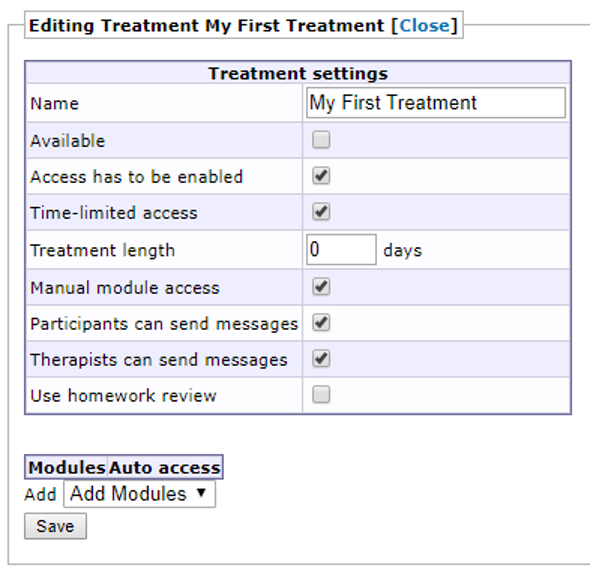
\includegraphics{images/new-images/treatmentTreatSettings.png}

Before adding in modules with content to the treatment, there are a few \textbf{Treatment settings} to consider.

\textbf{Available}
By checking this box, the treatment can be assigned to participants.

\begin{quote}
\textbf{Important note:} Any participants assigned to the treatment will automatically and continuously have access to all its content unless you limit the access with the settings below.
\end{quote}

\textbf{Access has to be enabled/time-limited access}
If the \emph{Access has to be enabled} box is checked, the treatment has to be manually activated for a participant before its content becomes available to that participant.

By also checking the \emph{Time-limited access} box, you can specify a time window for a participant when the treatment is active and its content available. This time window is specified in the participant view, under the \textbf{Treatments} tab.

\textbf{Treatment length}
If the treatment is to be available for a certain numbre of days after it has been activated, you can set that value in the \emph{Treatment length} box. You can always override/customize the treatment availability for a specific paricipant in the \textbf{Treatment access} tab of the participant.

\textbf{Manual model access}
Check this box to be able to activate each module in the treatment separately for a participant. This is useful for when you want to make sure participants are finished with one module before starting with the next one.

\textbf{Participants can send messages}
Checking this box makes it possible for participants to send messages to their therapists during an active treatment, by using the built-in messaging feature in BASS.

\textbf{Therapists can send messages}
Checking this box makes it possible for therapists to send messages to their participants during an active treatment, by using the built-in messaging feature in BASS.

\textbf{Use homework review}
Checking this box has two implications:

\begin{itemize}
\tightlist
\item
  First, a participant can choose to either save a homework (to be able to work on it later), or send it to the therapist (which marks it as finished and locks it, disabling further editing).
\item
  Second, an icon will be displayed i the \emph{Homework} column of the \emph{Participant search} view, that flags whenever a participant has submitted a finished homework and thus notifies the therapists of the fact at a glance.
\end{itemize}

\textbf{Modules}
This is where you connect modules to your treatment. If you have not yet created any modules this will be empty, without any modules to choose from.
If you're working in an established database with pre-existing treatment modules, they will show up in the dropdown menu. Click on a treatment module to add it to your treatment.

\textbf{Pages}
This option lets you add a \emph{treatment content} as a separate menu page in the participant's view. For example, this could be a sleep diary which the participants are to work with for the duration of their treatment, or any similar worksheet that is not part of any particular module. It may also be an instructions page, or a page with a collection of links to downloadable treatment content, such as a PDF document.

\textbf{Welcome screen}
Here, you may type in content to show a custom welcome screen/home page in the participant's view. There are a handful of instructions given on the page itself, to show conditional text or content.
For example, by using the \texttt{\textless{}ongoing\textgreater{}*YourContentHere*\textless{}/ongoing\textgreater{}} tag, you can specify the content enclosed in that tag to show when the treatment is ongoing. This is, in essence, the standard text for your home page.
By using \texttt{\textless{}daysleft\textgreater{}*YourContentHere*\textless{}/daysleft\textgreater{}} you can set content to show only as long as the participant has more than one day left of the treatment. When that time has passed, this content will not be shown.
By using \texttt{\textless{}lastday\textgreater{}*YourContentHere*\textless{}/lastday\textgreater{}} you can set the content to only show on the last day of access. This might be a thank you and/or good luck text, or something similar or appropriate for your treatment.
By using \texttt{\textless{}limited\textgreater{}*YourContentHere*\textless{}/limited\textgreater{}} you can set content to only show when the participant has only limited access to the treatment. For example, this could simply be a text informing the participant of the limited access and the changed it entails.
Using \texttt{\textless{}limiteddaysleft\textgreater{}*YouContentHere*\textless{}/limiteddaysleft\textgreater{}} you can set conditional content to be shown as long as the participant has more than one day left of their limited access.
Using \texttt{\textless{}limitedlastday\textgreater{}*YourContentHere*\textless{}/limitedlastday\textgreater{}} you can set conditional content to be shown on the participant's last day of limited acces, such as thanking them for their time and effort, and whishing them good luck.

\hypertarget{treatment-modules}{%
\section{Treatment Modules}\label{treatment-modules}}

Now, let's create modules for our treatment. To do this, click \emph{Close} at the top of the page to exit the treatment settings and return to the Treatment view for your treatment. Here, click the dropdown menu at the bottom of the page and select Module. You will be taken to the settings page for the module. Here, you can give it a name, and tags if you wish. Below these two boxes, there are three dropdown menus:

\begin{enumerate}
\def\labelenumi{\arabic{enumi}.}
\tightlist
\item
  \textbf{Main text} is where you assign a treatment content to be the main text of the module. This is usually the instructions, a psycho-educational text and other information relevant to the module.
\item
  \textbf{Worksheets} is where you assign a treatment content to be a worksheet connected to the module. You can assign multiple worksheets to a single module. Worksheets can be worked with and iterated upon by the participant.
\item
  \textbf{Homework} is where you assign a treatment content to be the homework of the module. You may only assign one homework per module. Homework can not be iterated upon by the participant once it has been submitted for review and subsequently approved by the therapist. If the therapist returns the homework to the participant, they're able to make changes.
\end{enumerate}

If you're working in a newly created databasa, leave the main text, worksheets, and homework dropdown menus empty, since there is no \emph{treatment content} to assign yet.
If you're working in a pre-existing treatment with completed \emph{treatment content} ready for use, add them as appropriate.
Click \emph{Close} at the top of the Module settings page to close it and return to the treatment overview.

\hypertarget{treatment-content}{%
\section{Treatment Content}\label{treatment-content}}

So, let's create some treatment content to add to our module. The treatment content is where most of the work goes into treatments. This is where you add text content, media content, forms and other input fields. You have a large degree of freedom to design your own treatment content and you can have it be as simple or as advanced you want or your knowledge of \textbf{HTML}, \textbf{CSS}, and if you're an advanced user, \textbf{JavaScript} dictates. We will be including some templates of the most commonly used \textbf{HTML} in this manual that you can copy and paste into your treatment content. To build a ``complete'' module with main text, one worksheet, and a homework, we'll need to create three separate treatment content units.

We will start by creating the main text one and work onwards from there in a ``bottom up'' fashion where we lay the foundation first, and add the complementary content when that's done.

\begin{enumerate}
\def\labelenumi{\arabic{enumi}.}
\tightlist
\item
  So, to add a treatment content navigate to your treatment if you're not already there. From the Create new dropdown menu at the bottom of the page, select treatment content. This will take you to the settings and editing page of the treatment content. Start by giving it an appropriate name in the box labeled Name at the top, and click \emph{Save}.
\item
  You may add tags if you wish, to make the content searchable.
\item
  \emph{Data namespace} is recommended to leave as is (auto-generated) unless you have a clear and specific reason to change it. The name space is used by BASS to identify the treatment content and save the information contained within in.
\item
  \emph{Path to file} lets you assign a file to be the content of the treatment content instead of a text. By clicking the Browse server button you will be taken to the internal file manager of your BASS database, from where you can set up a folder structure. This server browser is somewhat limited in comparison to the insert link version in that you cannot upload any files through this version, only select already existing files to link to.
\item
  \emph{Show example content} lets you fill in a worksheet example to see how a worksheet is built in BASS. Click Fill in example in BASS4 below to view an example version of a worksheet from the participant point of view.
\item
  \emph{Use markdown+HTML (else only HTML)} lets you decide whether to use HTML and Markdown for formatting, or only \textbf{HTML}. We recommend leaving this checked, unless you're confident in your \textbf{HTML} skills and do not wish to have any Markdown syntax potentially interfering in your \textbf{HTML} code.
\item
  Navigation mode is a new option added to treatment content that lets you select the manner in which your content is presented. Click the corresponding radio button to select the mode you wish to use.

  \begin{itemize}
  \tightlist
  \item
    \emph{Indexed by H1 tags} is the default option and presents the content as a long continuously scrollable page. You can visually divide it into cards by using the \textbf{HTML} tag \texttt{\textless{}h1\textgreater{}YourHeading\textless{}/h1\textgreater{}}, or by using the Markdown syntax \#YourHeading.
  \item
    \emph{Split into pages (use \texttt{\textbackslash{}PAGEBREAK} at the top level)} lets you divide the content into individual pages, PowerPoint-style. As per the instruction in the option text, use \texttt{\textbackslash{}PAGEBREAK} where you wish to insert a page break and switch to a new page.
  \end{itemize}
\item
  Content can be completed multiple times using tabs\ldots{} lets you use the div element with class=''tabbed'' as following \texttt{\textless{}div\ class=”tabbed”\textgreater{}*YourContent*\textless{}/div\textgreater{}}, to have for example a weekly diary be repeatable beyond the first week, without having to set up 10 individual weeks by coding them by hand. The participant can simply click a plus sign to add a new tab, with a fresh week ready to be filled in.
\end{enumerate}

\hypertarget{content-text}{%
\subsection{Content text}\label{content-text}}

Content text is the main editing window where you add the text, media content, forms and input field etc. to your treatment content. This is all formatted and structured through Markdown and/or \textbf{HTML}.
A few things are worth knowing when working with \textbf{HTML} in BASS:

\begin{enumerate}
\def\labelenumi{\arabic{enumi}.}
\tightlist
\item
  You do not need to define the document type (\texttt{\textless{}!—DOCTYPE\ HTML\ -\/-\textgreater{}})
\item
  You do not need to use \texttt{\textless{}html\textgreater{}}, \texttt{\textless{}head\textgreater{}}, \texttt{\textless{}title\textgreater{}} or \texttt{\textless{}body\textgreater{}}.
\item
  You do not need to define any CSS styles, since BASS has its own \textbf{CSS} sheet that will be the standard design for your treatment content. If you do want to have custom \textbf{CSS} styles for part of your treatment, you can use the \texttt{\textless{}style\textgreater{}} tag to insert those CSS rules and apply them. Do note however, that you may only apply \textbf{CSS} styles to elements within your treatment content. You cannot apply styles to BASS itself.
\end{enumerate}

Now, creating content is as simple as starting to type into the edit box. It may seem daunting at first if you are unfamiliar with \textbf{Markdown} and \textbf{HTML}, but there are several good resources available on the web.
One good resource for Markdown is found here: \url{https://www.markdownguide.org}.
A good resource for HTML is found here: \url{https://www.w3schools.com}.
If you want to perform advanced actions, such as automated calculations using user input as variables, you will need to learn some \textbf{JavaScript}, and add it to your treatment content with the \texttt{\textless{}script\textgreater{}} tag.

A typical start of a module main text may look as follows when written in \textbf{Markdown}:

\begin{Shaded}
\begin{Highlighting}[]
\NormalTok{“# Welcome to your treatment!}

\NormalTok{This is a ten-week treatment during which we will work together and learn about your symptoms and diagnosis. We will begin this week with psycho-educational material, and continue with some practical breathing exercises. The module should take about 20-30 minutes to complete. It is important that your read all the instructions carefully so that you feel you understand completely. Should you have any questions you are welcome to send us a message by using the “Messages” feature at the top of the page.}
\NormalTok{If you encounter any errors, please use the “Problems?” feature on the top right hand side.}

\NormalTok{Your treatment is divided into ten weeks, with a new module each week. Talk to your therapist if you feel you need to go slower. The modules are as follows:}
\NormalTok{- }\FloatTok{Module 1, start and information}
\FloatTok{- Module 2}
\FloatTok{- Module 3}
\FloatTok{- Module 4}
\FloatTok{- Module 5}
\FloatTok{- Module 6}
\FloatTok{- Module 7}
\FloatTok{- Module 8}
\FloatTok{- Module 9}
\FloatTok{- Module 10, finish”}
\end{Highlighting}
\end{Shaded}

The same main text written in HTML would look like this:

\begin{Shaded}
\begin{Highlighting}[]
\NormalTok{“}\KeywordTok{<h1>}\NormalTok{Welcome to your treatment!}\KeywordTok{</h1>}

\NormalTok{This is a ten-week treatment during which we will work together and learn about your symptoms and diagnosis. We will begin this week with psycho-educational material, and continue with some practical breathing exercises. The module should take about 20-30 minutes to complete. It is important that your read all the instructions carefully so that you feel you understand completely. Should you have any questions you are welcome to send us a message by using the “Messages” feature at the top of the page.}
\NormalTok{If you encounter any errors, please use the “Problems?” feature on the top right hand side.}

\NormalTok{Your treatment is divided into ten weeks, with a new module each week. Talk to your therapist if you feel you need to go slower. The modules are as follows:}

\KeywordTok{<ul>}
  \KeywordTok{<li>}\NormalTok{Module 1, start and information}\KeywordTok{</li>}
  \KeywordTok{<li>}\NormalTok{Module 2}\KeywordTok{</li>}
  \KeywordTok{<li>}\NormalTok{Module 3}\KeywordTok{</li>}
  \KeywordTok{<li>}\NormalTok{Module 4}\KeywordTok{</li>}
  \KeywordTok{<li>}\NormalTok{Module 5}\KeywordTok{</li>}
  \KeywordTok{<li>}\NormalTok{Module 6}\KeywordTok{</li>}
  \KeywordTok{<li>}\NormalTok{Module 7}\KeywordTok{</li>}
  \KeywordTok{<li>}\NormalTok{Module 8}\KeywordTok{</li>}
  \KeywordTok{<li>}\NormalTok{Module 9}\KeywordTok{</li>}
  \KeywordTok{<li>}\NormalTok{Module 10, finish}\KeywordTok{</li>}
\KeywordTok{</ul>}\NormalTok{”}
\end{Highlighting}
\end{Shaded}

Here we've used a heading (\texttt{\#} in \textbf{Markdown}, \texttt{\textless{}h1\textgreater{}} in \textbf{HTML}), then written some informative text, and finished with an unordered, i.e non-numbered, list (\texttt{-} in \textbf{Markdown}, \texttt{\textless{}ul\textgreater{}} and \texttt{\textless{}li\textgreater{}} in \textbf{HTML}). You can create ordered, i.e numbered, lists by using numbers in place of the dash in \textbf{Markdown}, or using \texttt{\textless{}ol\textgreater{}} in place of \texttt{\textless{}ul\textgreater{}} in \textbf{HTML}. Refer to the guides and tutorials linked above for further information on syntax and formatting in \textbf{Markdown} and/or \textbf{HTML}.

Below the edit box are three buttons. The \emph{Save} button does what it says on the tin: it saves your work. Make a habit of saving often.
Then there are two more buttons: \emph{Insert link} and \emph{Preview}.

The Preview button will preview your saved treatment content, to give you an idea of how it will look to the participants. It's very useful for checking that your design looks as intended, and as a quick way to check your progress. We recommend that you also create a dummy participant for which you activate your treatment, so that you can log into that participant account and check that your treatment works and looks good ``live'', so to speak.

Note that when you click \emph{Save}, your Preview window will be emptied. Simply click \emph{Preview} again to show your preview.
The \emph{Insert link} button will take you to the file manager in BASS once clicked (the file manager will open in a new browser tab). Here you can upload images, audio and video files, documents and so on, to be used in your treatment content or be made available to download for your participants. At the top of the page you will see the file path you're currently in.

It is good practice to set up an easily navigable folder structure before you start uploading any files. Click the \emph{Create new folder} button at the bottom of the page to create a new folder. Note that any new folder you create will be created within the folder you're currently located in (i.e if you've created folder A and then navigated/clicked into it and create folder B, folder B will be created within folder A). The reason we're doing this in advance is that you cannot move files around once they've been uploaded, so it is important that they are uploaded to their proper place from the start.

Once you've set up your folder structure, make sure you are in the folder you want the file to be uploaded to, and go to the lower edge of the screen and click \emph{Välj fil} (Swedish for Select file). This will bring up a file browser, showing local files on your computer, where you can navigate to and select the file you want to upload from your computer. Once you've found the correct file, select it and click \emph{Överför} (Swedish for Transfer, or Submit). You may also double-click the file. Once you've done so, you will be back at the file manage in BASS, and can see the name of the file you've selected for upload at the bottom of the page. If it is the correct file, go to the bottom right corner of the window and click Upload. Depending on the size of the file, this might take a moment. When the upload is finished, your file will be visible in the file manager window. Simply click it to add its file path to your treatment content.

Now, depending on the type of file you've uploaded, you will need to use different \textbf{Markdown syntax} or \textbf{HTML tags} to have to show in your treatment content.

If it is an image file, you will need to use the following Markdown syntax:
\texttt{!{[}My\ Image{]}(image.png)}

If you'd rather write HTML, you use the following tag:

\begin{Shaded}
\begin{Highlighting}[]
\KeywordTok{<img}\OtherTok{ src=}\StringTok{”image.png”}\KeywordTok{>}
\end{Highlighting}
\end{Shaded}

The ``image.png'' is used here as a placeholder for the file path to your image. As such, it should be replaced and will look something like this: \texttt{File.php?uploadedfile=/{[}file\ path\ to\ your\ image{]}}.

If it is an audio file, you will have to use \textbf{HTML} since \textbf{Markdown} does not handle audio files.

\begin{Shaded}
\begin{Highlighting}[]
\KeywordTok{<audio}\OtherTok{ controls}\KeywordTok{>}
  \KeywordTok{<source}\OtherTok{ src=}\StringTok{"audio.mp3"}\OtherTok{ type=}\StringTok{"audio/mp3"}\KeywordTok{>}
\KeywordTok{</audio>}
\end{Highlighting}
\end{Shaded}

As with audio, \textbf{Markdown} does not handle video files so you will have to use \textbf{HTML} for video files as well. The \textbf{HTML} is similar to that which is used for audio, but refers to video instead. see the example below.

\begin{Shaded}
\begin{Highlighting}[]
\KeywordTok{<video}\OtherTok{ controls}\KeywordTok{>}
  \KeywordTok{<source}\OtherTok{ src=}\StringTok{”video.mp4”}\OtherTok{ type=}\StringTok{”video/mp4”}\KeywordTok{>}
\KeywordTok{</video>}
\end{Highlighting}
\end{Shaded}

As with the image example above, the ``audio.mp3'' and ``video.mp4'' examples given here are just placeholder, and should be replaced with the actual file path to your audio or video file.

One very common \textbf{HTML} tag to use is \texttt{\textless{}textarea\textgreater{}}. This will let you create a text input box where participant can write answers to questions.
To use this simply type:

\begin{Shaded}
\begin{Highlighting}[]
\KeywordTok{<textarea}\OtherTok{ name=}\StringTok{”textarea1”}\KeywordTok{></textarea>}
\end{Highlighting}
\end{Shaded}

A very important part of any type of input you add to your treatment document, is to give it a unique \emph{``name''-attribute}. This unique name may not be shared by any other \textbf{HTML} element within the same treatment content. This is because the \emph{name-attribute} is used by BASS to differentiate between inputs and the answers that participants give. If you use the same \emph{name-attribute} for several \textbf{HTML} elements, they will be filled in with the same answer when a participant clicks save, overwriting any other answers given.

Another common \textbf{HTML tag} to use is \texttt{\textless{}table\textgreater{}}. This is very useful to structure content into columns and rows.
A table is a little more complex than a textarea, and consists of three main \textbf{HTML tags}, as follows:

\begin{Shaded}
\begin{Highlighting}[]
\KeywordTok{<table>}
  \KeywordTok{<tr>}
    \KeywordTok{<td>}
\NormalTok{      *Your content*}
    \KeywordTok{</td>}
  \KeywordTok{</tr>}
\KeywordTok{</table>}
\end{Highlighting}
\end{Shaded}

The \texttt{\textless{}table\textgreater{}} tag defines where your table begins and where it ends. The \texttt{\textless{}tr\textgreater{}} tag is a table row, and creates and closes table rows. The \texttt{\textless{}td\textgreater{}} tag is table data, i.e a table cell within a row. You can use multiple \texttt{\textless{}td\textgreater{}} tags within a

tag to create multiple cells.
One last mention on tables: tables in BASS are by default scrollable horizontally, to allow you to build wide tables if needed. If you do not wish your table to be scrollable, add \texttt{class=”non-scrollable”} to the \texttt{\textless{}table\textgreater{}} tag, like this:

\begin{Shaded}
\begin{Highlighting}[]
\KeywordTok{<table}\OtherTok{ class=}\StringTok{”non-scrollable”}\KeywordTok{>}
  \KeywordTok{<tr>}
    \KeywordTok{<td>}
\NormalTok{      *Your content*}
    \KeywordTok{</td>}
  \KeywordTok{</tr>}
\KeywordTok{</table>}
\end{Highlighting}
\end{Shaded}

BASS features \emph{basic syntax highlighting}, and will color different parts of your \textbf{HTML}, \textbf{CSS} and \textbf{JavaScript} code to make it easier to read and find elements of your code. In addition, if you've forgotten to close an HTML tag, it will be colored bright red to remind you and highlight potential problems within your code.

If you're working with a lot of \textbf{HTML} in your treatment contents, it may benefit you to check your code regularly in a dedicated coding program (known as an IDE), such as Atom \url{https://atom.io} or Visual Studio Code \href{https://code.visualstudio.com}{https://codde.visualstudio.com}. These programs are specifically designed to write code, and will give you a good overview of your entire document.

This covers the basic of building treatment content in BASS. We recommend you play around with it while referencing the resources linked above. If you run into issues, feel free to contact us.

\textbf{To add a treatment content} as either a main text, a homework, or a worksheet, go back to the treatment overview and click Edit next to the module you created. In the settings view that opens up, select the appropriate dropdown menu (main text, homework, worksheet) and select your treatment content from the list. Click Save.

\hypertarget{references}{%
\chapter{References}\label{references}}

In this chapter we list some helpful references and tools that might aid you when working with BASS.

\hypertarget{tools-and-resources-for-working-with-treatments}{%
\section{Tools and resources for working with treatments}\label{tools-and-resources-for-working-with-treatments}}

Treatments are the most complex and knowledge-intensive thing to build and maintain within BASS, as they require some know-how when it comes to \textbf{Markdown} and \textbf{HTML}. If you want to add some stylish flair to your treatment, you'll need to dive into a bit of \textbf{CSS}.
More advanced and more interactive treatments might require knowledge of \textbf{JavaScript} as well. Here below are some online resources and tools which you may find helpful:

\textbf{Coding software (IDE:s)}

\begin{itemize}
\tightlist
\item
  \url{https://atom.io} (an open-source IDE with good enthusiast support)
\item
  \url{https://code.visualstudio.com} (a full-featured IDE from Microsoft)
\end{itemize}

\textbf{Online resources on Markdown, HTML, and JavaScript}

\begin{itemize}
\tightlist
\item
  \url{https://www.markdownguide.org} (a well presented and comprehensive guide on using Markdown)
\item
  \url{https://www.w3schools.com} (a good resource for referencing HTML, CSS and JavaScript)
\item
  \url{https://javascript.info} (an in-depth and comprehensive guide and tutorial on JavaScript)
\end{itemize}

\bibliography{bibliography.bib,packages.bib}

\end{document}
